% adapted by WS from SSR's Word document and from the 5-part series at
% https://www.overleaf.com/learn/latex/How_to_Write_a_Thesis_in_LaTeX_(Part_1):_Basic_Structure
% reviewed by MAM

\documentclass[12pt,twosided]{report}

\usepackage[titletoc]{appendix} % for adding appendix to TOC
\usepackage{biblatex}  % reference management
\usepackage{geometry}  % better margins and margin control
\usepackage{graphicx}  % to include figures
\usepackage{hyperref}  % internal and external links
\usepackage[utf8]{inputenc}  % support for non-ASCII characters
\usepackage{listings}  % typset code
\usepackage{outlines}  % easy nesting of lists
\usepackage{tabularx}  % more control over table column width
\usepackage{titlesec}  % customize chapter title 
\usepackage{upquote}  % prevent mishandling of single quotes in listings


% TODO: Customize the appearance of hyperref links using \hypersetup
% See https://en.wikibooks.org/wiki/LaTeX/Hyperlinks#Customization

% Custom format of chapter title.
\titleformat{\chapter}[hang]{\bf\huge}{\thechapter.}{2pc}{}

% Separate folder for images named 'images'.
\graphicspath{ {images/} }

% Separate file for references
\addbibresource{references.bib}

% Replace with your title
\title{NeuroHire: AI-Driven Recruitment Booth}

% Allow recalling document title
% from https://tex.stackexchange.com/a/15806/44301
\makeatletter\let\Title\@title\makeatother  

\begin{document}

\include{titlepage}  % title page.
\include{approval}  % approval page.

\chapter*{Dedication}
We dedicate this project to our parents and families, whose unwavering support, patience, and encouragement have been the foundation of our academic journey. Their belief in us has continuously motivated us to strive for excellence and overcome every challenge along the way.

We extend our sincere gratitude to our mentors and instructors for their guidance, valuable insights, and continuous support throughout the development of this project. Their mentorship played a crucial role in shaping our understanding and helping us translate our ideas into a practical and meaningful system.

This project is especially dedicated to individuals seeking employment in mass hiring environments, particularly those with limited or no formal skills. Such candidates are often evaluated through processes that are inconsistent and time-consuming. NeuroHire is built with the aim of improving large-scale recruitment by introducing a more structured, efficient, and unbiased approach to candidate evaluation, ensuring that individuals are assessed based on their responses and behavior during the screening process.

We hope this work contributes toward improving hiring practices and supports organizations in making faster and more consistent recruitment decisions at scale.

Lastly, we acknowledge the dedication, collaboration, and perseverance of our team members, whose combined efforts made the successful completion of this project possible.

\chapter*{Acknowledgements}
We would like to express our sincere gratitude to the Computer Science faculty for providing us with the knowledge, resources, and environment necessary to carry out this project successfully.

We are especially thankful to our supervisor, Professor Ahsan Javed, for his continuous guidance, support, and valuable feedback throughout the development of this project. His insights and mentorship played a crucial role in shaping our approach and improving the overall quality of our work.

We would also like to extend our appreciation to KFC for their support in providing us with relevant data and for facilitating user testing. Their cooperation allowed us to evaluate our system in a more practical and realistic setting, which significantly contributed to the effectiveness of our solution.

Lastly, we acknowledge the efforts of everyone who directly or indirectly contributed to the completion of this project.

\chapter*{Abstract}
Recruitment for mass hiring roles can be challenging, with organizations often required to evaluate large volumes of candidates within limited timeframes. The process is not only time-consuming but also prone to inconsistencies that can affect decision-making. NeuroHire seeks to address this by providing an intelligent, AI-driven solution to automate the initial screening and evaluation of candidates.

The system enables candidates to upload their CVs and record structured video responses to predefined interview questions. CVs are processed using optical character recognition (OCR), while video responses are analyzed through speech transcription and computer vision techniques. Instead of relying solely on manual review, NeuroHire evaluates candidate responses based on relevance, clarity, confidence, and behavioral indicators such as eye contact and head movement. The platform also incorporates video quality checks to ensure the reliability of inputs and flags uncertain cases for further review.

Designed to support large-scale recruitment environments, NeuroHire provides a structured scoring mechanism that helps standardize candidate evaluation while significantly reducing manual workload. The system does not replace human recruiters but assists them by presenting organized insights and scores, enabling more informed and efficient decision-making. By combining automation with human oversight, NeuroHire aims to make hiring faster, more consistent, and better suited for high-volume recruitment scenarios.

% The following are automatically populated by LaTeX \chapter, \section and related, \figure, and \table.
\tableofcontents
\listoffigures
\listoftables

\chapter{Introduction}
\label{chap:intro}
\section{Problem Statement}
Recruitment and selection are critical processes for every organization, yet traditional hiring practices are often time-consuming, labor-intensive, and prone to inconsistency. Recruiters must manually review large numbers of CVs, shortlist candidates, conduct interviews, and compare applicants across multiple criteria. This becomes even more difficult in remote and high-volume hiring settings, where the number of applicants can exceed the capacity of human evaluators.

Recent advances in artificial intelligence have improved several parts of the recruitment pipeline, such as resume screening, interview automation, and candidate matching. However, many existing systems address only isolated tasks. Some focus mainly on resume parsing, others on speech recognition, while some analyze visual or behavioral cues from interviews. This fragmentation creates a gap in practical hiring systems, since recruiters often need a unified view of candidate suitability rather than separate outputs from disconnected tools.

Another challenge is that hiring decisions are not based only on qualifications written in a CV. Spoken responses, communication quality, clarity of answers, and observable behavioral cues during interviews may also provide useful information. Existing approaches often do not combine these dimensions in a structured and interpretable way. Moreover, concerns related to fairness, transparency, and reliability remain important when artificial intelligence is applied in recruitment.

Therefore, the problem addressed in this project is the lack of an integrated and explainable recruitment support system that can analyze candidate information from multiple modalities, including CVs, interview speech, and behavioral video cues, in a single framework.

\section{Proposed Solution}
To address this problem, this project proposes \textbf{NeuroHire}, an AI-assisted recruitment support system for multimodal candidate evaluation. The system is designed to assist recruiters by combining three major capabilities within a unified pipeline.

First, NeuroHire performs \textbf{CV analysis} to extract and organize relevant candidate information, enabling structured screening of resumes. This helps reduce the manual effort required in early-stage shortlisting and supports more consistent initial evaluation.

Second, the system performs \textbf{speech-based interview analysis}. Candidate responses from video interviews are transcribed and processed to assess their relevance to the given interview question, along with qualities such as clarity and confidence. This enables the system to move beyond simple transcription and support structured understanding of candidate responses.

Third, NeuroHire includes \textbf{behavioral video analysis} to observe cues such as gaze direction, head movement, and facial stability during interviews. These cues are not treated as final indicators on their own, but as supportive signals that can help assess engagement and interview interaction behavior.

The outputs of these modules are combined into a structured evaluation framework that supports decision-making for recruiters. In addition, the system includes quality checks so that poor video conditions, such as blur or inadequate lighting, can be flagged for human review. In this way, NeuroHire aims to provide a more comprehensive and practical recruitment aid than systems that focus on only one stage of hiring.

\section{Intended User}
NeuroHire is designed for a multi-user recruitment environment involving candidates, recruiters, companies, and a super admin. Each user type interacts with the system according to its specific role in the hiring process.

\textbf{Candidate:}  
The candidate is one of the primary users of the system. A candidate interacts with NeuroHire by selecting a preferred language for the interview, uploading a CV, selecting an available job, reviewing submitted information, and recording a video interview response. This allows the system to collect the required data for CV-based screening, speech analysis, and behavioral evaluation.

\textbf{Recruiter:}  
Recruiters use the system to manage recruitment activities related to their organization. Their responsibilities include adding, editing, and deleting job postings, reviewing applicants for posted jobs, and monitoring statistics related to jobs and applicants. Recruiters can also report issues or submit error-related complaints through the system when necessary.

\textbf{Company:}  
The company user supervises recruiter-level activity within the platform. A company can manage recruiters by accepting or rejecting recruiter registrations and can review overall statistics related to recruitment activity. This role helps ensure that only authorized recruiters are allowed to operate under the company’s account.

\textbf{Super Admin:}  
The super admin is responsible for platform-level administration. This user manages companies by accepting or rejecting company registrations and can review system-wide statistics. The super admin ensures overall control, governance, and proper onboarding of organizations using the platform.

Overall, NeuroHire is intended for a structured hiring ecosystem in which each user type contributes to a different stage of the recruitment and administration process.

\section{Project gantt chart and deliverables}
Please include a detailed gantt and details of the deliverables for Kaavish I and II

\section{Key Challenges}
The development of NeuroHire involves several important challenges.

One major challenge is \textbf{multimodal integration}. NeuroHire combines CV analysis, speech-based response evaluation, and behavioral video analysis within a single system. Since these modules process different types of input data, their outputs must be integrated carefully so that the final evaluation remains meaningful, consistent, and easy to interpret. This challenge can be addressed by designing the system using a modular architecture, where each component performs its own task independently and then passes structured outputs to a central scoring or decision layer.

Another challenge is \textbf{speech transcription accuracy}. Since the system relies on transcription of interview responses before evaluating answer relevance, clarity, and confidence, any error in speech recognition may affect downstream analysis. This issue becomes more significant in multilingual settings, varied accents, or noisy environments. A possible way to address this challenge is to use a robust speech recognition model, support controlled interview conditions, and include preprocessing or confidence-based checks before passing the transcript to later stages of analysis.

The system also faces challenges in \textbf{behavioral cue interpretation}. Signals such as gaze direction, blinking, facial stability, or head movement can provide useful indicators of candidate engagement and interaction behavior, but they should not be treated as direct proof of candidate suitability or dishonesty. These cues may be influenced by environmental conditions, camera placement, internet quality, or natural individual differences in behavior. This challenge can be addressed by treating behavioral features as supportive indicators only, rather than final decision variables, and by allowing uncertain cases to be flagged for human review.

Another important challenge is \textbf{video quality and environmental variability}. Since NeuroHire depends on video input for behavioral analysis, poor lighting, blurred frames, low-resolution webcams, or unstable internet connections may reduce the reliability of extracted visual features. To address this issue, the system can include video quality checks such as blur detection and lighting assessment, and discard or down-weight unreliable behavioral scores when the input quality falls below acceptable thresholds.

A further challenge is \textbf{fairness and explainability}. AI-based recruitment systems may raise concerns if their outputs are difficult to understand or if users believe the system may introduce bias. This is especially important in hiring contexts, where trust and transparency are essential. A possible way to address this challenge is to design NeuroHire as a decision-support system rather than a fully autonomous decision-maker, and to provide structured score components that help recruiters understand how the system reached its evaluation.

Finally, \textbf{user trust and practical adoption} remain important challenges. Even if the system performs well technically, recruiters and organizations may hesitate to rely on it unless it aligns with real hiring workflows and produces understandable results. This challenge can be addressed by ensuring that the system output is simple, interpretable, and aligned with practical recruitment needs, while keeping human decision-makers involved in the final hiring process.

\chapter{Literature Review}
\label{chap:lit}
% \chapter{Literature Review}

% \section{Introduction}
% Artificial intelligence has increasingly been applied in recruitment and selection to improve efficiency, reduce manual workload, and support data-driven decision-making. Existing work in this domain spans several important areas, including automated resume screening, AI-assisted interview evaluation, speech recognition, behavioral analysis, and fairness in algorithmic hiring. While these developments have significantly advanced the state of the art, many existing approaches focus on only one stage of the recruitment pipeline. Since NeuroHire is designed as an integrated recruitment support system, it is important to review literature from each of these related domains and examine how prior work aligns with, or differs from, the proposed system.

\section{AI in Recruitment and Selection}
Artificial intelligence has been widely explored as a means of improving recruitment workflows. Rathore discusses the impact of AI on recruitment and selection processes and explains that AI can automate repetitive tasks such as resume screening, interview scheduling, and candidate communication, thereby improving efficiency and reducing manual workload for recruiters \cite{rathore_ai_recruitment}. The study also places these developments in the broader context of electronic human resource management, where digital platforms support online recruitment and virtual selection processes.

Similarly, Sha Ri examines the application of artificial intelligence in recruitment and selection, with emphasis on resume screening, interviewing, and competency assessment \cite{sha_ri_ai_recruitment}. The study explains that natural language processing can be used to extract candidate information from resumes, while machine learning and data mining can support matching between candidates and job requirements. It further highlights the role of speech recognition and computer vision in analyzing candidate responses and non-verbal behavior during interviews.

These studies demonstrate that AI has become an important part of modern recruitment systems. However, they mainly discuss the role of AI at a general level and do not present a complete multimodal framework that combines CV analysis, interview response understanding, and behavioral evaluation in a single end-to-end system. This motivates the need for an integrated system such as NeuroHire.

\section{Bias, Fairness, and Transparency in Algorithmic Hiring}
As AI systems become more common in hiring, fairness and transparency have emerged as major concerns. Raghavan \textit{et al.} analyze publicly available claims made by vendors of algorithmic hiring tools and show that many of these systems rely on question-based assessments, video interview analysis, and game-based evaluations \cite{raghavan2020bias}. Their study identifies significant shortcomings in transparency, especially regarding model validation and the fairness-related claims made by vendors.

A major concern raised in this work is that many algorithmic hiring systems depend on historical employee data. Because such data may reflect previous organizational bias, predictive models risk reproducing unfair patterns instead of reducing them \cite{raghavan2020bias}. The authors also argue that fairness is often treated in a limited way, for example through compliance-based measures, without addressing deeper issues in the data and modeling process.

This literature is important for NeuroHire because it highlights that hiring systems should not be treated as opaque decision-makers. Instead, they should provide structured and interpretable outputs. Unlike many black-box hiring tools criticized in prior work, NeuroHire is intended as a decision-support system that combines automated analysis with human-readable score components and the possibility of human review.

\section{Speech Recognition for Interview Systems}
Speech recognition is a foundational component of AI-assisted interview analysis. Radford \textit{et al.} propose a large-scale weakly supervised speech recognition approach trained on approximately 680,000 hours of multilingual and multitask audio data \cite{radford2022whisper}. Their work demonstrates strong robustness and generalization across multiple benchmarks and shows that performance improves significantly with increasing training scale and diversity. The study also supports multilingual transcription and translation, which is especially relevant for interview settings where candidates may respond in different languages.

This work is highly relevant to NeuroHire because accurate transcription is necessary before candidate responses can be analyzed for relevance, clarity, and confidence. However, the role of speech recognition in NeuroHire goes beyond general transcription. While Radford \textit{et al.} focus on robust speech recognition itself, NeuroHire uses transcription as an enabling step for structured interview response evaluation in a recruitment context.

\section{Multimodal Interview Assessment}
A growing body of research supports the use of multimodal AI for automated interview evaluation. In \textit{Automated Analysis and Prediction of Job Interview Performance}, the authors propose a framework for quantifying verbal and non-verbal behaviors in interview settings using prosodic, lexical, and facial features \cite{naim2015jobinterview}. Their results show that higher speaking rate, fewer filler words, and more positive language are associated with better interview performance. The study also demonstrates that multimodal analysis outperforms single-modality approaches in predicting interview-related traits.

Nguyen \textit{et al.} study body communication cues in employment interviews and show that gestures, posture, and speaking status can be used to predict hirability and personality-related outcomes \cite{nguyen2013bodycommunication}. Their work emphasizes that non-verbal behavior is closely linked with speech and contributes significantly to interview outcomes. However, the study also notes that part of the analysis depends on manual annotations, which limits full automation.

Zhang \textit{et al.} further extend this area by investigating asynchronous video interviews and proposing a multimodal framework for assessing personality traits and interview performance using visual, audio, and verbal signals \cite{zhang2025avi}. Their work addresses limitations in earlier studies by using a structured interview dataset designed for realistic job application scenarios and annotated by trained evaluators. The proposed baseline combines visual, audio, and textual representations and shows that multimodal systems can improve prediction performance in interview assessment tasks.

These studies strongly support the use of multimodal signals in video interview analysis. However, most of them focus on predictive modeling, dataset creation, or benchmarking rather than developing a practical recruitment support system. NeuroHire differs by using multimodal analysis within a larger system that also includes CV analysis, job-specific screening, and structured scoring for deployment-oriented candidate evaluation.

\section{Behavioral Analysis}
Behavioral signals such as gaze direction, blinking, and head movement are often used as indicators of attention and interaction behavior. Pimplaskar \textit{et al.} propose a real-time eye blinking detection and tracking system using OpenCV and show that eye-related visual cues can be extracted effectively under real-time conditions \cite{pimplaskar2013eye}. Their work demonstrates the practical feasibility of monitoring eye activity using computer vision methods and highlights the broader relevance of eye-based cues for attention-related analysis.

Head pose is another important visual signal. Huttunen \textit{et al.} study computer vision methods for head pose estimation and show that machine learning approaches can achieve strong performance in predicting yaw and pitch from facial images despite challenges such as limited data, illumination changes, and label ambiguity \cite{huttunen_headpose}. Their work provides technical support for using head orientation as a measurable behavioral feature.

For NeuroHire, these studies justify the use of gaze-related and head-pose-related signals as part of behavioral analysis during interviews. At the same time, such cues must be interpreted carefully. In NeuroHire, they are intended to act as supportive indicators of engagement and interaction behavior rather than standalone measures of competence or honesty.

\section{Existing AI-Based Interview Systems}
Some prior systems are relatively close to the goals of NeuroHire. Pandey \textit{et al.} propose an AI-based interview system that combines speech recognition, facial expression analysis, resume parsing, and machine learning-based evaluation \cite{pandey2025aibased}. Their system uses natural language processing for content-related analysis, OpenCV and convolutional neural networks for visual analysis, and a composite scoring mechanism to generate overall interview performance scores.

This work demonstrates that combining textual, vocal, and visual analysis in recruitment systems is both feasible and useful. However, NeuroHire differs in several ways. It is designed as a more structured multimodal recruitment framework rather than a collection of loosely connected modules. In addition, NeuroHire places stronger emphasis on explainable scoring, system-level integration, and controlled use of behavioral cues within a broader recruitment support pipeline.

\section{Discussion and Relevance to NeuroHire}
The literature reviewed in this chapter shows that substantial progress has been made in AI-based recruitment, speech recognition, multimodal interview analysis, and behavioral video assessment. Prior work supports the use of AI for resume screening and recruitment automation \cite{rathore_ai_recruitment,sha_ri_ai_recruitment}, robust multilingual transcription \cite{radford2022whisper}, multimodal prediction of interview performance \cite{naim2015jobinterview,nguyen2013bodycommunication,zhang2025avi}, and extraction of visual behavioral cues such as eye movement and head pose \cite{pimplaskar2013eye,huttunen_headpose}. At the same time, literature on algorithmic hiring highlights concerns related to fairness, transparency, and interpretability \cite{raghavan2020bias}.

A key observation from the reviewed work is that many existing approaches address only one part of the hiring process at a time. Some focus on recruitment automation at a high level, some on transcription, and others on multimodal interview prediction or behavioral feature extraction. Comparatively fewer systems attempt to combine CV analysis, speech-based answer evaluation, behavioral analysis, and structured decision support in one coherent framework.

This is where NeuroHire establishes its contribution. Rather than treating candidate evaluation as a single prediction task, NeuroHire integrates multiple modalities into a unified recruitment support pipeline. It combines CV-based screening, speech transcription and response analysis, and behavioral signal extraction from interview videos, while also emphasizing explainable outputs and practical usability. In this way, NeuroHire builds upon the strengths of prior work while addressing the lack of integration among existing approaches.



\chapter{Software Requirement Specification (SRS)}
\label{chap:srs}
This chapter provides detailed specifications of the system under development.

\section{Functional Requirements}
% ─────────────────────────────────────────────────────────────────────────────

This section describes the functional requirements of the NeuroHire system, organised by
user role as reflected in the system's use case diagrams. Each requirement describes a
discrete, implementable behaviour that the system must support.

\begin{outline}

  \1 \textbf{Candidate Module:}

  \2 \textbf{FR-C1 -- Language Selection:}
  The system shall allow a candidate to select their preferred interface language (Urdu or
  English) at the start of every session. All subsequent on-screen text, audio prompts, and
  guidance shall be rendered in the selected language.

  \2 \textbf{FR-C2 -- Voice Guidance:}
  The system shall provide an optional voice guidance mode in which all instructions and
  prompts are delivered through audio output, enabling candidates with limited literacy to
  navigate the application process independently.

  \2 \textbf{FR-C3 -- View Job Listings:}
  The system shall display all active job postings assigned to the current recruitment pod,
  allowing a candidate to browse available positions and select one before beginning their
  application.

  \2 \textbf{FR-C4 -- CV Upload:}
  The system shall capture a candidate's curriculum vitae either by scanning a physical
  document. The uploaded CV shall be stored and linked to
  the candidate's application record.

  \2 \textbf{FR-C5 -- Review Extracted CV Information:}
  Upon successful CV capture, the system shall perform OCR-based text extraction and present
  the parsed information to the candidate for review. The candidate shall be able to correct
  any inaccuracies in the extracted data before submission.

  \2 \textbf{FR-C6 -- Record Video Interview:}
  The system shall guide the candidate through a structured video recording session
  comprising job-specific screening questions, and shall upload the recorded video responses
  to the backend upon completion.

    \3 \textbf{FR-C6a -- Answer Screening Questions:}
    During the recording session, the system shall present each job-specific screening
    question defined by the recruiter, prompting the candidate to respond on camera before
    proceeding to the next question.

    \3 \textbf{FR-C6b -- Upload Video Responses:}
    The system shall upload the completed video responses to backend storage upon session
    completion. A progress indicator shall inform the candidate of upload status and provide
    a retry option in case of failure.

  \2 \textbf{FR-C7 -- Receive Submission Confirmation:}
    Upon successful submission of the CV and video responses, the system shall display a
    confirmation message acknowledging that the application has been received and is under
    review.

  \2 \textbf{FR-C8 -- Video Quality Feedback:}
  The system shall evaluate the quality of the recorded video submission.
  \1 \textbf{Recruiter Module:}

  \2 \textbf{FR-R1 -- Login and Signup:}
  The system shall provide secure authentication for recruiters, supporting both new account
  registration and login for existing accounts. Access to the dashboard shall be granted only
  upon successful authentication. New accounts shall remain in a pending state until approved
  by the associated Company user.

  \2 \textbf{FR-R2 -- Post Vacancies:}
  The system shall allow recruiters to create new job postings, each comprising a job
  description and a set of screening questions configured by the recruiter.

    \3 \textbf{FR-R2a -- Add Job Description:}
    When creating a vacancy, the system shall allow the recruiter to compose and save a
    detailed job description including role requirements.

    \3 \textbf{FR-R2b -- Add Screening Questions:}
    The system shall allow recruiters to define a list of video-based screening questions for
    each job posting, which shall be presented to candidates during the video recording stage
    at the pod.

    \3 \textbf{FR-R2c -- Edit Job Posting:}
    The system shall allow recruiters to edit any field of an existing job posting, including
    description, and screening questions. Changes shall take effect
    immediately for future applications.

    \3 \textbf{FR-R2d -- Activate and Deactivate Jobs:}
    The system shall allow recruiters to toggle a job posting's status between active and
    inactive. Inactive jobs shall not be displayed to candidates at the pod and shall not
    accept new applications.

    \3 \textbf{FR-R2e -- Delete Job Posting:}
    The system shall allow recruiters to permanently remove a job posting from active views
    via a soft-delete, retaining associated application records and AI assessments for audit.

    \3 \textbf{FR-R2f -- Set Scoring Threshold:}
    The system shall allow recruiters to configure a minimum composite score threshold for a
    job. Candidates whose scores fall below this threshold shall be flagged or ranked
    accordingly in the applicant list.

  \2 \textbf{FR-R3 -- View Applicants:}
  The system shall present recruiters with a ranked list of candidates who have applied for
  a specific job, ordered by composite AI score.

    \3 \textbf{FR-R3a -- View CV:}
    The system shall provide access to the parsed CV data and the original uploaded CV
    document for each candidate within the applicant view.

    \3 \textbf{FR-R3b -- View Video Interviews:}
    The system shall allow recruiters to play back recorded video responses submitted by a
    candidate directly within the dashboard.

    \3 \textbf{FR-R3c -- View AI Recommendation:}
    The system shall display the AI-generated composite score and recommendation (Accept,
    Reject, or Send to Human Interview) for each candidate application.

    \3 \textbf{FR-R3d -- Filter and Search Applicants:}
    The system shall allow recruiters to filter the applicant list by score range, submission
    language, and review status (including the ``Needs HR Review'' tag). Applied filters shall
    update the candidate table in real time.

  \2 \textbf{FR-R4 -- Make Hiring Decision:}
  The system shall allow recruiters to record a final hiring decision for each applicant,
  which may agree with or override the AI recommendation. The decision shall be persisted in
  the recruiter decisions log.

    \3 \textbf{FR-R4a -- Accept Candidate:}
    The system shall allow a recruiter to mark a candidate as accepted, updating the
    application status accordingly.

    \3 \textbf{FR-R4b -- Reject Candidate:}
    The system shall allow a recruiter to reject a candidate, recording the decision and any
    associated comments in the recruiter decisions log.

    \3 \textbf{FR-R4c -- Send to Human Interview:}
    The system shall allow a recruiter to forward a candidate to a human interview stage when
    further evaluation is required beyond the automated AI assessment.

    \3 \textbf{FR-R4d -- Add Notes and Flags:}
    The system shall allow recruiters to attach free-text notes and a flag marker to any
    application record, enabling documentation of reasoning for team reference or future
    handover.

  \2 \textbf{FR-R5 -- Report System Errors:}
  The system shall provide a mechanism for recruiters to report technical issues or system
  errors encountered during use. Reports shall be logged and made available for Super Admin
  review.

  \2 \textbf{FR-R6 -- Edit Recruiter Profile:}
  The system shall allow a recruiter to update their own account details, including full
  name, email address, and password. Password changes shall require confirmation of the
  current password and shall enforce minimum strength criteria.

  \1 \textbf{Company / Head of HR Module:}

  \2 \textbf{FR-CO0 -- Company Signup and Login:}
  The system shall provide secure account registration and login for Company users. A new
  company registration shall remain in a pending state until approved by the Super Admin.
  Login shall enforce authentication and session management consistent with other roles.

  \2 \textbf{FR-CO1 -- Manage Recruiters:}
  The system shall allow the Company to manage all recruiter accounts associated with their
  organisation, including the ability to approve, disable, and delete recruiter accounts.

    \3 \textbf{FR-CO1a -- Approve Recruiters:}
    The system shall allow the Company to approve a recruiter account, granting that recruiter
    access to the dashboard and the ability to manage job postings.

    \3 \textbf{FR-CO1b -- Disable Recruiters:}
    The system shall allow the Company to temporarily disable a recruiter account, preventing
    access without permanently removing the account or its data.

    \3 \textbf{FR-CO1c -- Delete Recruiters:}
    The system shall allow the Company to permanently delete a recruiter account and its
    associated data from the organisation.

  \2 \textbf{FR-CO2 -- View All Jobs:}
  The system shall provide the Company with a consolidated view of all active and inactive
  job postings created by recruiters within their organisation.

  \2 \textbf{FR-CO3 -- View Applicants Overview:}
  The system shall provide the Company with an aggregated overview of applicant activity
  across all job postings, allowing high-level visibility into recruitment progress.

  \2 \textbf{FR-CO4 -- Report an Issue:}
  The system shall provide the Company with a mechanism to report operational or technical
  issues to the Super Admin for resolution and tracking.

  \2 \textbf{FR-CO5 -- Update Company Profile:}
  The system shall allow the Company user to update their organisation's profile information,
  including company name, logo, and primary contact details. Logo changes shall be reflected
  in booth branding within one synchronisation cycle.

  \2 \textbf{FR-CO6 -- View Audit Log:}
  The system shall provide the Company with a read-only audit log of all recruiter decisions
  and significant actions performed within their organisation, including action type, job
  title, candidate identifier, and timestamp. The log shall be filterable by recruiter, job,
  and date range.

  \1 \textbf{Super Admin Module:}

  \2 \textbf{FR-SA1 -- View Platform Overview:}
  The system shall provide the Super Admin with a high-level dashboard displaying key
  operational metrics and the current health status of the platform, including total
  registered companies, active recruiters, and applications processed.

  \2 \textbf{FR-SA2 -- View Recruiter Error Log:}
  The system shall allow the Super Admin to access a log of all system errors reported by
  or associated with recruiter activity.

  \2 \textbf{FR-SA3 -- View Company Error Log:}
  The system shall allow the Super Admin to access a log of all system errors reported by
  or associated with company-level accounts.

  \2 \textbf{FR-SA4 -- Change Error Status:}
  The system shall allow the Super Admin to update the resolution status of any logged error,
  marking it as either Resolved or Unresolved to track issue management progress.

  \2 \textbf{FR-SA5 -- Manage Companies:}
  The system shall allow the Super Admin to manage all company accounts registered on the
  platform, including the ability to approve, reject, and delete company accounts.

    \3 \textbf{FR-SA5a -- Approve Company:}
    The system shall allow the Super Admin to approve a company registration request,
    granting that company access to the NeuroHire platform and enabling its recruiters to
    begin operations.

    \3 \textbf{FR-SA5b -- Reject Company:}
    The system shall allow the Super Admin to reject a company registration request,
    preventing the company from accessing the platform.

    \3 \textbf{FR-SA5c -- Delete Company:}
    The system shall allow the Super Admin to permanently delete a company account and all
    associated recruiter accounts and data from the platform.

  \2 \textbf{FR-SA6 -- Configure Platform Settings:}
  The system shall allow the Super Admin to configure global platform settings, including
  default AI scoring thresholds, supported languages, and quality-check parameters, through
  a settings console without requiring a code deployment. All changes shall be validated
  before saving and a configuration change history shall be maintained.

\end{outline}

% ─────────────────────────────────────────────────────────────────────────────
\subsection{User Stories}
\label{sec:user-stories}
% ─────────────────────────────────────────────────────────────────────────────

The following table presents the user stories derived from the system use case diagrams,
mapped to their corresponding functional requirements. Stories are organised into four epics
aligned with the four human roles in the system. The \textbf{FR~Ref.} column
cross-references each story to the functional requirement(s) it realises, ensuring full
traceability between stakeholder needs and system behaviour.

% ── Colour and badge definitions (scoped to this file) ───────────────────────
\definecolor{nhHeader}{RGB}{45,55,110}
\definecolor{nhEpic1}{RGB}{221,232,255}
\definecolor{nhEpic2}{RGB}{214,245,226}
\definecolor{nhEpic3}{RGB}{255,240,214}
\definecolor{nhEpic4}{RGB}{236,222,255}
\definecolor{nhRow1}{RGB}{240,244,255}
\definecolor{nhRow2}{RGB}{240,255,245}
\definecolor{nhRow3}{RGB}{255,250,240}
\definecolor{nhRow4}{RGB}{250,240,255}
\definecolor{nhHighBg}{RGB}{255,224,224}
\definecolor{nhHighFg}{RGB}{163,32,32}
\definecolor{nhMedBg}{RGB}{255,240,204}
\definecolor{nhMedFg}{RGB}{122,80,0}
\definecolor{nhLowBg}{RGB}{214,245,214}
\definecolor{nhLowFg}{RGB}{26,92,26}
\definecolor{nhEpic1txt}{RGB}{26,45,122}
\definecolor{nhEpic2txt}{RGB}{13,92,48}
\definecolor{nhEpic3txt}{RGB}{122,69,0}
\definecolor{nhEpic4txt}{RGB}{75,26,122}

\newcommand{\High}{\colorbox{nhHighBg}{\textcolor{nhHighFg}{\textbf{\footnotesize High}}}}
\newcommand{\Med}{\colorbox{nhMedBg}{\textcolor{nhMedFg}{\textbf{\footnotesize Med}}}}
\newcommand{\Low}{\colorbox{nhLowBg}{\textcolor{nhLowFg}{\textbf{\footnotesize Low}}}}

% ── The table is placed in a landscape environment so it fits A4 ─────────────

\setlength{\arrayrulewidth}{0.4pt}
\setlength{\tabcolsep}{4pt}
\renewcommand{\arraystretch}{1.3}

\scriptsize
\begin{longtable}{|p{0.8cm}|p{1.0cm}|p{1.2cm}|p{1.4cm}|p{4.2cm}|p{4.2cm}|p{1.8cm}|}
\caption{NeuroHire -- User Story Table (32 Stories, 4 Epics)}
\label{tab:user_stories}\\

\hline
\rowcolor{nhHeader}
\textcolor{white}{\textbf{US ID}} &
\textcolor{white}{\textbf{Epic}} &
\textcolor{white}{\textbf{Role}} &
\textcolor{white}{\textbf{User Type}} &
\textcolor{white}{\textbf{User Story}} &
\textcolor{white}{\textbf{Acceptance Criteria}} &
\textcolor{white}{\textbf{Module}} \\
\hline
\endfirsthead

\multicolumn{7}{c}{\tablename\ \thetable{} \textit{-- continued from previous page}}\\[3pt]
\hline
\rowcolor{nhHeader}
\textcolor{white}{\textbf{US ID}} &
\textcolor{white}{\textbf{Epic}} &
\textcolor{white}{\textbf{Role}} &
\textcolor{white}{\textbf{User Type}} &
\textcolor{white}{\textbf{User Story}} &
\textcolor{white}{\textbf{Acceptance Criteria}} &
\textcolor{white}{\textbf{Module}} \\
\hline
\endhead

\hline \multicolumn{7}{r}{\textit{Continued on next page $\longrightarrow$}}\\
\endfoot

\hline
\endlastfoot

%=============================================================================
% EPIC 1 – CANDIDATE
%=============================================================================
\rowcolor{nhEpic1}
\multicolumn{7}{|l|}{\hspace{4pt}\textcolor{nhEpic1txt}{\textbf{EPIC-1 \quad Candidate Onboarding \& Submission}}}\\
\hline

\rowcolor{nhRow1}
US-01 & EPIC-1 & Candidate & Walk-in applicant &
As a candidate, I want to select my preferred language (Urdu or English) at the start of my session so that all instructions are presented in a language I understand. &
Language selector is the first screen at session start; applies to all on-screen text, audio guidance, and STT processing; can be changed before submission is confirmed. & Candidate Pod Interface \\
\hline

\rowcolor{nhRow1}
US-02 & EPIC-1 & Candidate & Walk-in applicant &
As a candidate, I want to enable voice guidance so that I can follow the booth instructions without relying solely on reading the screen. &
A voice-guidance toggle is available on the language selection screen; when enabled, all instructions and prompts are read aloud in the selected language throughout the session. & Candidate Pod Interface \\
\hline

\rowcolor{nhRow1}
US-03 & EPIC-1 & Candidate & Walk-in applicant &
As a candidate, I want to view all job listings at the booth so that I can choose the role I want to apply for. &
Pod displays all active jobs mapped to that booth; candidate can scroll, read descriptions, and confirm a selection before proceeding. & Candidate Pod Interface \\
\hline

\rowcolor{nhRow1}
US-04 & EPIC-1 & Candidate & Walk-in applicant &
As a candidate, I want to scan or upload my CV at the booth so that my qualifications are captured without needing a digital file. &
CV image is captured, auto-enhanced for OCR readability, and stored in \texttt{CV\_Data}; success confirmation shown before the next step. &
CV Capture \& OCR \\
\hline

\rowcolor{nhRow1}
US-05 & EPIC-1 & Candidate & Walk-in applicant &
As a candidate, I want to review and edit the information extracted from my CV so that any OCR errors are corrected before submission. &
Parsed fields (name, education, skills, experience) displayed in an editable form after OCR; confirmed values saved back to \texttt{CV\_Data.parsed\_keywords} before proceeding. &
CV Capture \& OCR \\
\hline

\rowcolor{nhRow1}
US-06 & EPIC-1 & Candidate & Walk-in applicant &
As a candidate, I want to record video responses to job-specific screening questions so that I can demonstrate my communication and soft skills. &
System presents each screening question in sequence; candidate records a response per question; video meets minimum length and audio-quality thresholds; stored in \texttt{Video\_Submissions}; candidate may re-record once per question. & Video Capture Module \\
\hline

\rowcolor{nhRow1}
US-07 & EPIC-1 & Candidate & Walk-in applicant &
As a candidate, I want my video responses to be uploaded and receive a submission confirmation so that I know my application has been successfully received. &
Video files uploaded with a progress indicator; confirmation screen shows job applied for, submission timestamp, and reference number; confirmation stored in \texttt{Candidate\_Logs}. & Video Capture Module \\
\hline

\rowcolor{nhRow1}
US-08 & EPIC-1 & Candidate & Walk-in applicant &
As a candidate, I want immediate feedback if my video or audio quality is too poor so that I can re-record before leaving the booth. &
Quality-control rule evaluates noise, lighting, and transcript confidence; if below threshold a retry prompt appears with a plain-language explanation; up to two retries allowed. & Quality Control Rule \\
\hline

%=============================================================================
% EPIC 2 – RECRUITER
%=============================================================================
\rowcolor{nhEpic2}
\multicolumn{7}{|l|}{\hspace{4pt}\textcolor{nhEpic2txt}{\textbf{EPIC-2 \quad Recruiter Workflow}}}\\
\hline

\rowcolor{nhRow2}
US-09 & EPIC-2 & Recruiter & Recruiter &
As a recruiter, I want to sign up and log in securely so that my account is linked to my organisation and candidate data is protected. &
Sign-up requires company name; account created with \texttt{status = pending} until approved by the Company user; login enforces JWT authentication; sessions expire after a configurable idle period. &
Auth \& Account Mgmt \\
\hline

\rowcolor{nhRow2}
US-10 & EPIC-2 & Recruiter & Recruiter &
As a recruiter, I want to create a new job posting with a description, eligibility requirements, and screening questions so that candidates are evaluated against the right criteria. &
Job form saves title, description, eligibility text, and at least one screening question to \texttt{Jobs} and \texttt{Job\_Questions}; job defaults to \texttt{inactive} until explicitly activated. & Job Management \\
\hline

\rowcolor{nhRow2}
US-11 & EPIC-2 & Recruiter & Recruiter &
As a recruiter, I want to edit an existing job posting so that I can correct or update requirements without creating a duplicate. &
Edit form pre-populates current values; changes saved immediately for future applications; existing applications retain a snapshot of original requirements. & Job Management \\
\hline

\rowcolor{nhRow2}
US-12 & EPIC-2 & Recruiter & Recruiter &
As a recruiter, I want to activate or deactivate a job so that the pod only shows roles currently open for applications. &
Toggle sets \texttt{job.status} to \texttt{active} or \texttt{inactive}; inactive jobs disappear from the pod list within one sync cycle; action written to \texttt{Recruiter\_Logs}. & Job Management \\
\hline

\rowcolor{nhRow2}
US-13 & EPIC-2 & Recruiter & Recruiter &
As a recruiter, I want to delete a job posting so that obsolete roles are permanently removed from active views. &
Soft-delete marks job as \texttt{deleted}; associated applications and AI assessments retained for audit; deleted jobs hidden from all non-admin views. & Job Management \\
\hline

\rowcolor{nhRow2}
US-14 & EPIC-2 & Recruiter & Recruiter &
As a recruiter, I want to set a scoring threshold for a job so that only candidates meeting the minimum AI score are surfaced in the shortlist. &
Threshold saved per job; candidates scoring below threshold filtered from the ranked shortlist view; threshold can be updated at any time and takes effect immediately. & Job Management \\
\hline

\rowcolor{nhRow2}
US-15 & EPIC-2 & Recruiter & Recruiter &
As a recruiter, I want to view applicants including their CV, video interview, and AI recommendation so that I have full context before making a decision. &
Ranked candidate table shows parsed CV summary, video playback link, STT transcript, behavioral score, and AI recommendation per applicant row. & Recruiter Dashboard \\
\hline

\rowcolor{nhRow2}
US-16 & EPIC-2 & Recruiter & Recruiter &
As a recruiter, I want to filter and search candidates by score range, language, or review tag so that I can manage my review queue efficiently. &
Filter controls update the candidate table in real time; combined filters are additive (AND logic). & Recruiter Dashboard \\
\hline

\rowcolor{nhRow2}
US-17 & EPIC-2 & Recruiter & Recruiter &
As a recruiter, I want to accept, reject, or forward a candidate to a human interview so that a formal decision is recorded for every application. &
Action buttons visible per application row; outcome stored in \texttt{Recruiter\_Decisions} with recruiter ID, timestamp, and optional override flag; action logged. & Recruiter Decisions \\
\hline

\rowcolor{nhRow2}
US-18 & EPIC-2 & Recruiter & Recruiter &
As a recruiter, I want to add written notes and flags to an application so that my reasoning is documented for future reference or team handover. &
Free-text notes field and flag toggle saved to \texttt{Recruiter\_Decisions}; notes visible to other authorised recruiters in the same company. & Recruiter Decisions \\
\hline

\rowcolor{nhRow2}
US-19 & EPIC-2 & Recruiter & Recruiter &
As a recruiter, I want to edit my own profile (name, email, password) so that my account details remain accurate. &
Profile edit form validates email format and password strength; confirmation email sent on save; old password required to set a new one. &
Auth \& Account Mgmt \\
\hline

\rowcolor{nhRow2}
US-20 & EPIC-2 & Recruiter & Recruiter &
As a recruiter, I want to report a system error or unexpected behaviour so that technical issues are escalated to the Super Admin. &
``Report Issue'' form captures error description and optional screenshot; creates an \texttt{Error\_Log} entry tagged with \texttt{recruiter\_id}; Super Admin is notified automatically. & Error Reporting \\
\hline

%=============================================================================
% EPIC 3 – COMPANY
%=============================================================================
\rowcolor{nhEpic3}
\multicolumn{7}{|l|}{\hspace{4pt}\textcolor{nhEpic3txt}{\textbf{EPIC-3 \quad Company (Head of HR) Management}}}\\
\hline

\rowcolor{nhRow3}
US-21 & EPIC-3 & Company & Head of HR / Company rep &
As a Company user, I want to sign up and log in securely so that our organisation can access NeuroHire and our data is protected. &
Sign-up captures company name, industry, and primary contact; account set to \texttt{pending} until Super Admin approves; login enforces JWT authentication; failed attempts are logged. &
Auth \& Account Mgmt \\
\hline

\rowcolor{nhRow3}
US-22 & EPIC-3 & Company & Head of HR / Company rep &
As a Company user, I want to approve, disable, or delete recruiter accounts within our organisation so that I control who acts on our behalf inside NeuroHire. &
Pending-approvals queue lists recruiter accounts awaiting authorisation; approve grants dashboard access; disable sets \texttt{status = inactive} without deleting data; delete permanently removes the account after a confirmation prompt; all actions logged. & Company Console \\
\hline

\rowcolor{nhRow3}
US-23 & EPIC-3 & Company & Head of HR / Company rep &
As a Company user, I want to view all job postings created by recruiters in our organisation so that I have full oversight of current recruitment activity. &
Jobs dashboard lists all active, inactive, and deleted jobs; filterable by status and recruiter; read-only for Company users. & Company Console \\
\hline

\rowcolor{nhRow3}
US-24 & EPIC-3 & Company & Head of HR / Company rep &
As a Company user, I want an aggregated overview of applicant activity across all our job postings so that I can monitor overall recruitment pipeline health. &
Overview aggregates total applications per job, shortlist counts, and pending recruiter decisions; data refreshes at least every 5 minutes. &
Analytics \& Reporting \\
\hline

\rowcolor{nhRow3}
US-25 & EPIC-3 & Company & Head of HR / Company rep &
As a Company user, I want to report a platform issue to NeuroHire so that it can be investigated and resolved by the Super Admin. &
``Report Issue'' form captures description and optional attachment; creates an \texttt{Error\_Log} entry tagged with \texttt{company\_id}; Company user can track issue status (open / in progress / resolved). & Error Reporting \\
\hline

\rowcolor{nhRow3}
US-26 & EPIC-3 & Company & Head of HR / Company rep &
As a Company user, I want to update our company profile (name, logo, contact details) so that our branding remains current across the platform. &
Profile edit form validates required fields; logo upload enforces size and format constraints; changes reflected in booth branding within one sync cycle; update logged. & Company Console \\
\hline

\rowcolor{nhRow3}
US-27 & EPIC-3 & Company & Head of HR / Company rep &
As a Company user, I want to view an audit log of all recruiter decisions and actions within our organisation so that I have full oversight and accountability. &
Audit log lists recruiter name, action type, job title, candidate ID, and timestamp; filterable by recruiter, job, and date range; read-only. &
Audit \& Logs \\
\hline

%=============================================================================
% EPIC 4 – SUPER ADMIN
%=============================================================================
\rowcolor{nhEpic4}
\multicolumn{7}{|l|}{\hspace{4pt}\textcolor{nhEpic4txt}{\textbf{EPIC-4 \quad Super Admin (NeuroHire Platform)}}}\\
\hline

\rowcolor{nhRow4}
US-28 & EPIC-4 & Super Admin & Super Admin &
As a Super Admin, I want a global platform overview showing all registered companies, active recruiters, and system health so that I can monitor platform-wide usage. &
Dashboard displays total companies (active / pending / suspended), total recruiters, total applications processed (daily/monthly), and system uptime; data exportable as CSV. & Super Admin Console \\
\hline

\rowcolor{nhRow4}
US-29 & EPIC-4 & Super Admin & Super Admin &
As a Super Admin, I want to view error logs reported by recruiters and Company users in separate views so that I can triage issues by their source efficiently. &
Two distinct log queues: Recruiter Error Log and Company Error Log; each shows reporter name, company, description, timestamp, and status; both support filtering by date and status. & Error Logs \\
\hline

\rowcolor{nhRow4}
US-30 & EPIC-4 & Super Admin & Super Admin &
As a Super Admin, I want to update the resolution status of any reported error so that reporters are kept informed and the issue backlog is managed. &
Status toggle updates the \texttt{Error\_Log} record to Resolved or Unresolved; resolution notes can be added; the reporting user is notified by email on status change. & Error Logs \\
\hline

\rowcolor{nhRow4}
US-31 & EPIC-4 & Super Admin & Super Admin &
As a Super Admin, I want to approve, reject, or delete company accounts so that the platform only hosts legitimate and active organisations. &
Approve sets \texttt{company.status = active}; reject sets status to \texttt{rejected} with a stated reason and notifies the company; delete permanently removes the company and all associated recruiter accounts after a confirmation prompt; all actions logged. & Super Admin Console \\
\hline

\rowcolor{nhRow4}
US-32 & EPIC-4 & Super Admin & Super Admin &
As a Super Admin, I want to configure global platform settings (e.g.\ default AI thresholds, supported languages) so that system-wide behaviour can be adjusted without a code deployment. &
Settings console exposes key-value pairs in \texttt{System\_Settings}; changes validated before saving; change history maintained; settings take effect on the next processing cycle. & System Settings \\
\hline

\end{longtable}

\normalsize

% reset table settings to defaults for rest of document
\setlength{\tabcolsep}{6pt}
\renewcommand{\arraystretch}{1.0}

% --- End of Functional Requirements

% --- The above is to be modified as per your project, e.g. a flat list if your system has limited functional requirements.

\section{Non-functional Requirements}
% ─────────────────────────────────────────────────────────────────────────────

Requirements are grouped by category and are grounded in the constraints and objectives of
the project.

\begin{outline}
  \1 \textbf{Usability:}
  \2 \textbf{NFR-U1 -- Bilingual Interface:} The candidate pod interface shall support both Urdu and English, with all on-screen text, prompts, and audio guidance rendered in the language selected by the candidate at session start. Switching language shall take effect immediately without restarting the session.
  \2 \textbf{NFR-U2 -- Low-Literacy Accessibility:} The candidate pod interface shall be navigable by users with limited literacy through the combined use of audio guidance, icons, and minimal written text. No candidate shall be required to read extended passages to complete an application.
  \2 \textbf{NFR-U3 -- Guided Application Flow:} The candidate interface shall present a linear, step-by-step workflow that prevents candidates from skipping mandatory stages. Progress indicators shall be visible at all times during the application.
  \2 \textbf{NFR-U4 -- Recruiter Dashboard Clarity:} The recruiter dashboard shall present candidate rankings, AI scores, and action controls in a single unified view, enabling a recruiter to review and action an application without navigating to more than two additional screens.

  \1 \textbf{Security:}
  \2 \textbf{NFR-S1 -- Role-Based Access Control:} The system shall enforce role-based access control across all interfaces. Candidates, Recruiters, Company/Head of HR, and Super Admin roles shall each have access only to the features and data permitted for their role. Unauthorised access attempts shall be rejected and logged.
  \2 \textbf{NFR-S2 -- Secure Data Transmission:} All data transmitted between the candidate pod, recruiter dashboard, admin console, and the backend server shall be encrypted using HTTPS/TLS. Plain-text transmission of candidate data shall not be permitted.
  \2 \textbf{NFR-S3 -- Candidate Data Privacy:} Candidate CVs, video recordings, and AI-generated scores shall be accessible only to authenticated recruiters and admins within the scope of their role. Raw media files shall not be publicly accessible via direct URLs.
  \2 \textbf{NFR-S4 -- Authentication:} Recruiter and admin accounts shall require password-based authentication before granting access to the dashboard or console. Passwords shall be stored as cryptographic hashes; plain-text storage is prohibited.

  \1 \textbf{Performance:}
  \2 \textbf{NFR-P1 -- AI Processing Turnaround:} Following the submission of a candidate's CV and video responses, the system shall complete the full AI assessment pipeline --- including OCR, speech-to-text transcription, and behavioural scoring --- and make results available on the recruiter dashboard within a targeted time of under five minutes per candidate under normal operating conditions.
  \2 \textbf{NFR-P2 -- Pod Responsiveness:} The candidate pod interface shall respond to user interactions within two seconds under normal network conditions. Loading times for job listings and guidance screens shall not exceed three seconds.
  \2 \textbf{NFR-P3 -- Video Upload Reliability:} The system shall handle video file uploads reliably, providing retry mechanisms in the event of transient network failure. A partially uploaded file shall not be accepted as a complete submission.

  \1 \textbf{Reliability:}
  \2 \textbf{NFR-R1 -- Error Logging and Auditability:} The system shall log all processing errors, recruiter actions, and administrative events with timestamps. Logs shall be retained and accessible to the Super Admin for auditing and issue resolution purposes.
  \2 \textbf{NFR-R2 -- Graceful Degradation:} In the event of an AI processing failure (e.g., unintelligible audio, corrupted video file), the system shall not discard the application. Instead, it shall tag the application for manual HR review and surface it on the recruiter dashboard with an appropriate status indicator.
  \2 \textbf{NFR-R3 -- Data Integrity:} Each submitted application shall be atomically linked to its associated CV data, video submission, AI assessment, and recruiter decision. Partial or orphaned records shall not be created during normal operation or recoverable failure states.

  \1 \textbf{Maintainability:}
  \2 \textbf{NFR-M1 -- Modular AI Pipeline:} The AI processing components --- CV parsing, speech-to-text, and behavioural analysis --- shall be implemented as independently deployable modules with well-defined interfaces, so that any single module can be updated or replaced without requiring changes to the others.
  \2 \textbf{NFR-M2 -- Configurable Scoring Parameters:} AI scoring weights, eligibility thresholds, and quality-check parameters shall be configurable without modifying source code, enabling administrators to tune system behaviour through configuration rather than deployment.

  \1 \textbf{Fairness and Inclusivity:}
  \2 \textbf{NFR-F1 -- Language Parity:} The system shall apply equivalent AI scoring criteria to Urdu-language and English-language submissions. Systematic score differentials attributable solely to language choice shall be identified and mitigated during model evaluation.
  \2 \textbf{NFR-F2 -- Standardised Candidate Experience:} All candidates accessing the system through a recruitment pod shall be presented with the same hardware environment, interface layout, and sequence of prompts, ensuring that no candidate is advantaged or disadvantaged by the evaluation setup itself.
  \2 \textbf{NFR-F3 -- Human Override Availability:} The system shall always preserve the recruiter's ability to override an AI recommendation. No AI decision shall be treated as final without the possibility of human review and intervention.
\end{outline}

\section{External Interfaces}

We expect every project to have at least of the following subsections. This section must be aligned with your project deliverables. Please consult with your project supervisor regarding which of the following section(s) you should include in your report

\subsection{User Interfaces}
This section includes our mockup screens and briefly explains them.

\subsection{Application Program Interface (API)}
NeuroHire integrates several libraries and APIs across its AI-based processing modules. In the \textbf{Behavior Analysis Module}, the system uses \textbf{OpenCV} and \textbf{MediaPipe}. OpenCV is used for video frame processing and visual feature extraction, while MediaPipe is used for face and landmark detection to support analysis of head movement, gaze-related behavior, and facial stability.

For speech-related functionality, the system uses models accessed through the \textbf{Hugging Face} ecosystem. In particular, Hugging Face is used to access and manage the \textbf{MMS Text-to-Speech (MMS-TTS)} and \textbf{Whisper} models, which support speech generation and speech recognition tasks respectively.

The backend communication interface of the system is implemented using \textbf{FastAPI}. FastAPI is used to expose RESTful endpoints between the frontend and backend services, and also to enable communication between the main project and the LLM models deployed on the \textbf{High Performance Computing (HPC)} environment. Through these API endpoints, the system can send candidate-related inputs to the hosted models and receive analysis results for further processing.

In addition, the system uses the \textbf{OpenAI API} for \textbf{Urdu-to-English webpage translation}. This helps support multilingual interaction and improves accessibility for users who need translated interface or content support.

Overall, these APIs and libraries allow the system to integrate computer vision, speech processing, LLM-based analysis, and backend communication within a unified recruitment platform.

\subsection{Hardware/Communication Interfaces}
Since NeuroHire is designed to support video-based interview assessment, the recruitment pods must include a set of essential input, output, and networking components to capture and transmit candidate data reliably.

\begin{itemize}
    \item \textbf{Camera and Microphone:} These components are required to record the candidate's video responses and clear audio during the interview session. The captured video supports facial and behavioral analysis, while the audio input is used for speech-to-text conversion and answer evaluation.

    \item \textbf{Screen and Speaker:} These components are used to display interview instructions, questions, and other interface elements to the candidate. The speaker provides audio guidance and feedback, which is especially useful in assisted or multilingual interview settings.

    \item \textbf{Internet Access:} A stable network connection is required to enable seamless communication between the recruitment pods and the cloud-based backend system. This allows uploaded CVs, recorded videos, transcripts, and analysis results to be transferred efficiently for storage and processing.
\end{itemize}

\section{Use Cases}
\subsection*{Interaction with Candidates}

\begin{figure}[H]
    \centering
    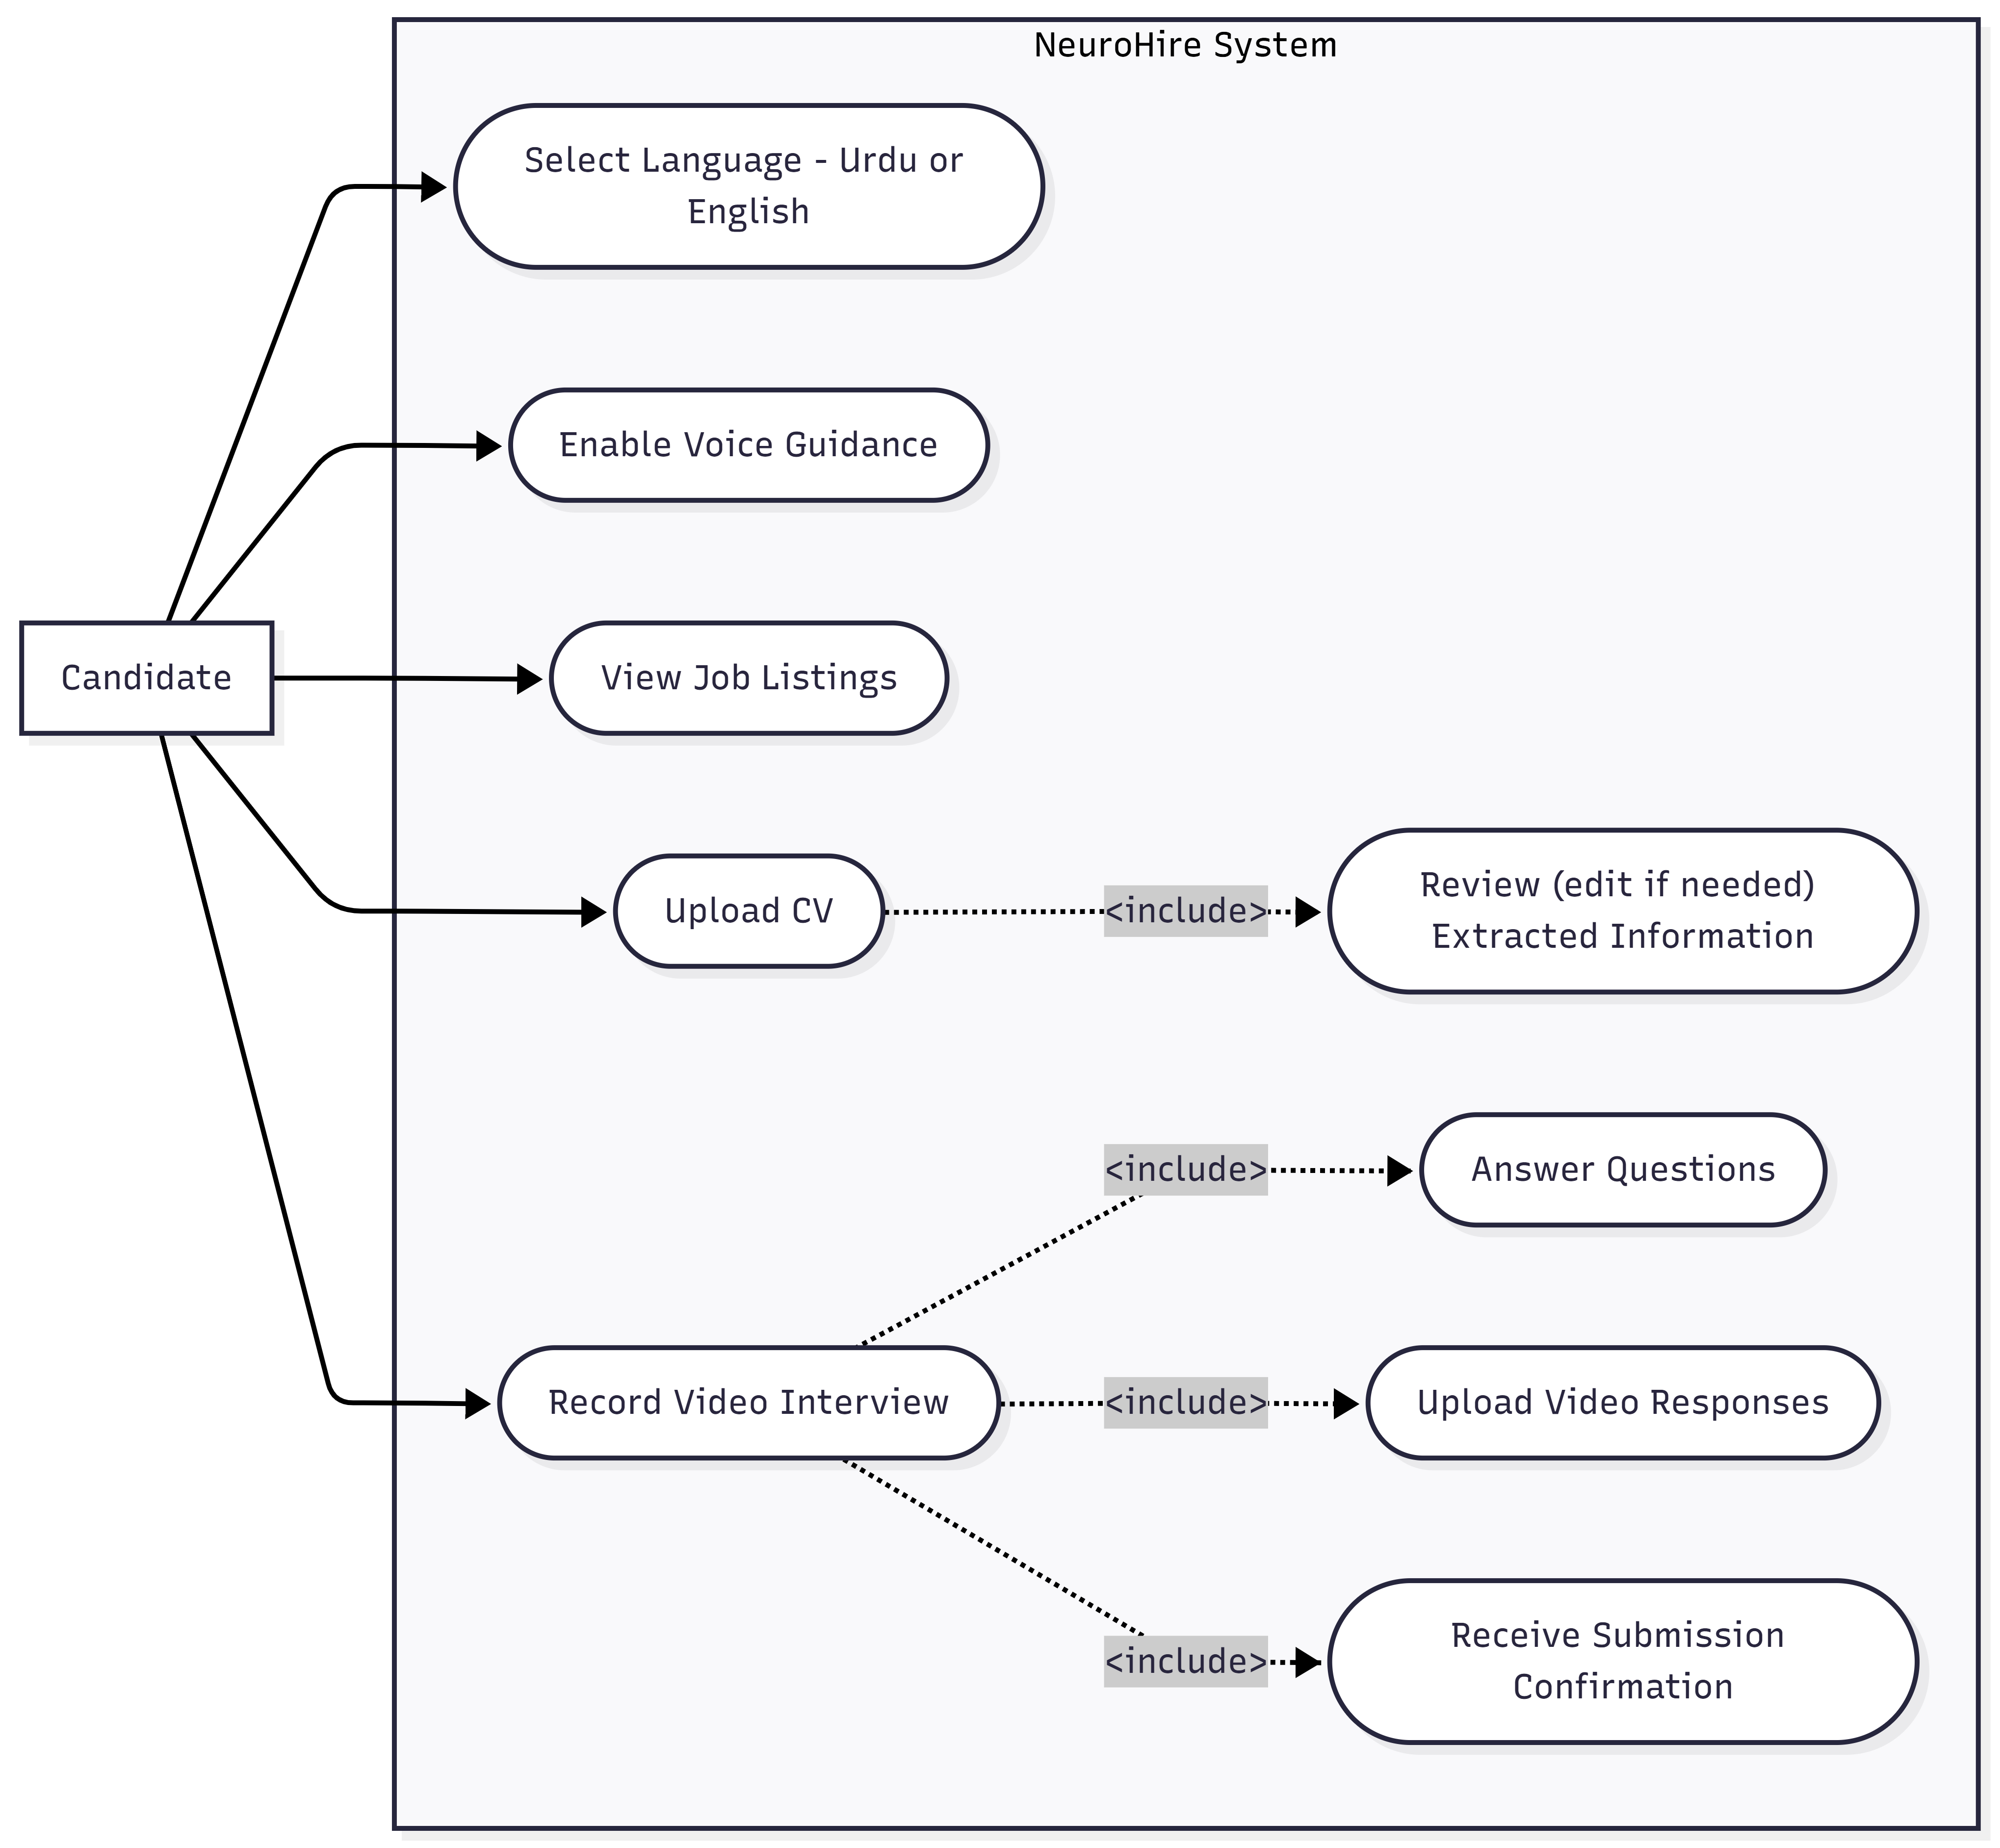
\includegraphics[width=\textwidth]{NeuroHire System Candidate-2026-04-11-144308.png}
    \caption{Candidate Use Case Diagram}
    \label{fig:neurohire-candidate-usecase}
\end{figure}

The use case diagram illustrates how a candidate interacts with the NeuroHire AI Recruitment System to explore job opportunities, submit application materials, and complete the interview process. The system is designed to be accessible, guided, and supportive for users applying to no-skill job roles. At the start of the interaction, the candidate can \textbf{select a preferred language (Urdu or English)} and \textbf{enable voice guidance}, improving accessibility and providing audio-based instructions for users with limited literacy or technical familiarity. The candidate can then \textbf{view job listings} to browse available opportunities and select suitable roles. To apply, the candidate must \textbf{upload a CV}, after which the system extracts relevant information such as education, skills, and experience; the candidate can \textbf{review and edit extracted information} to ensure accuracy before proceeding. A key stage of the process is the \textbf{video interview}, which includes mandatory sub-activities modeled using \texttt{<<include>>} relationships: \textbf{answering predefined questions}, \textbf{uploading video responses}, and \textbf{receiving submission confirmation}. These steps ensure a structured, consistent, and complete evaluation process for every candidate.

\subsection*{Interaction with Recruiters}

\begin{figure}[H]
    \centering
    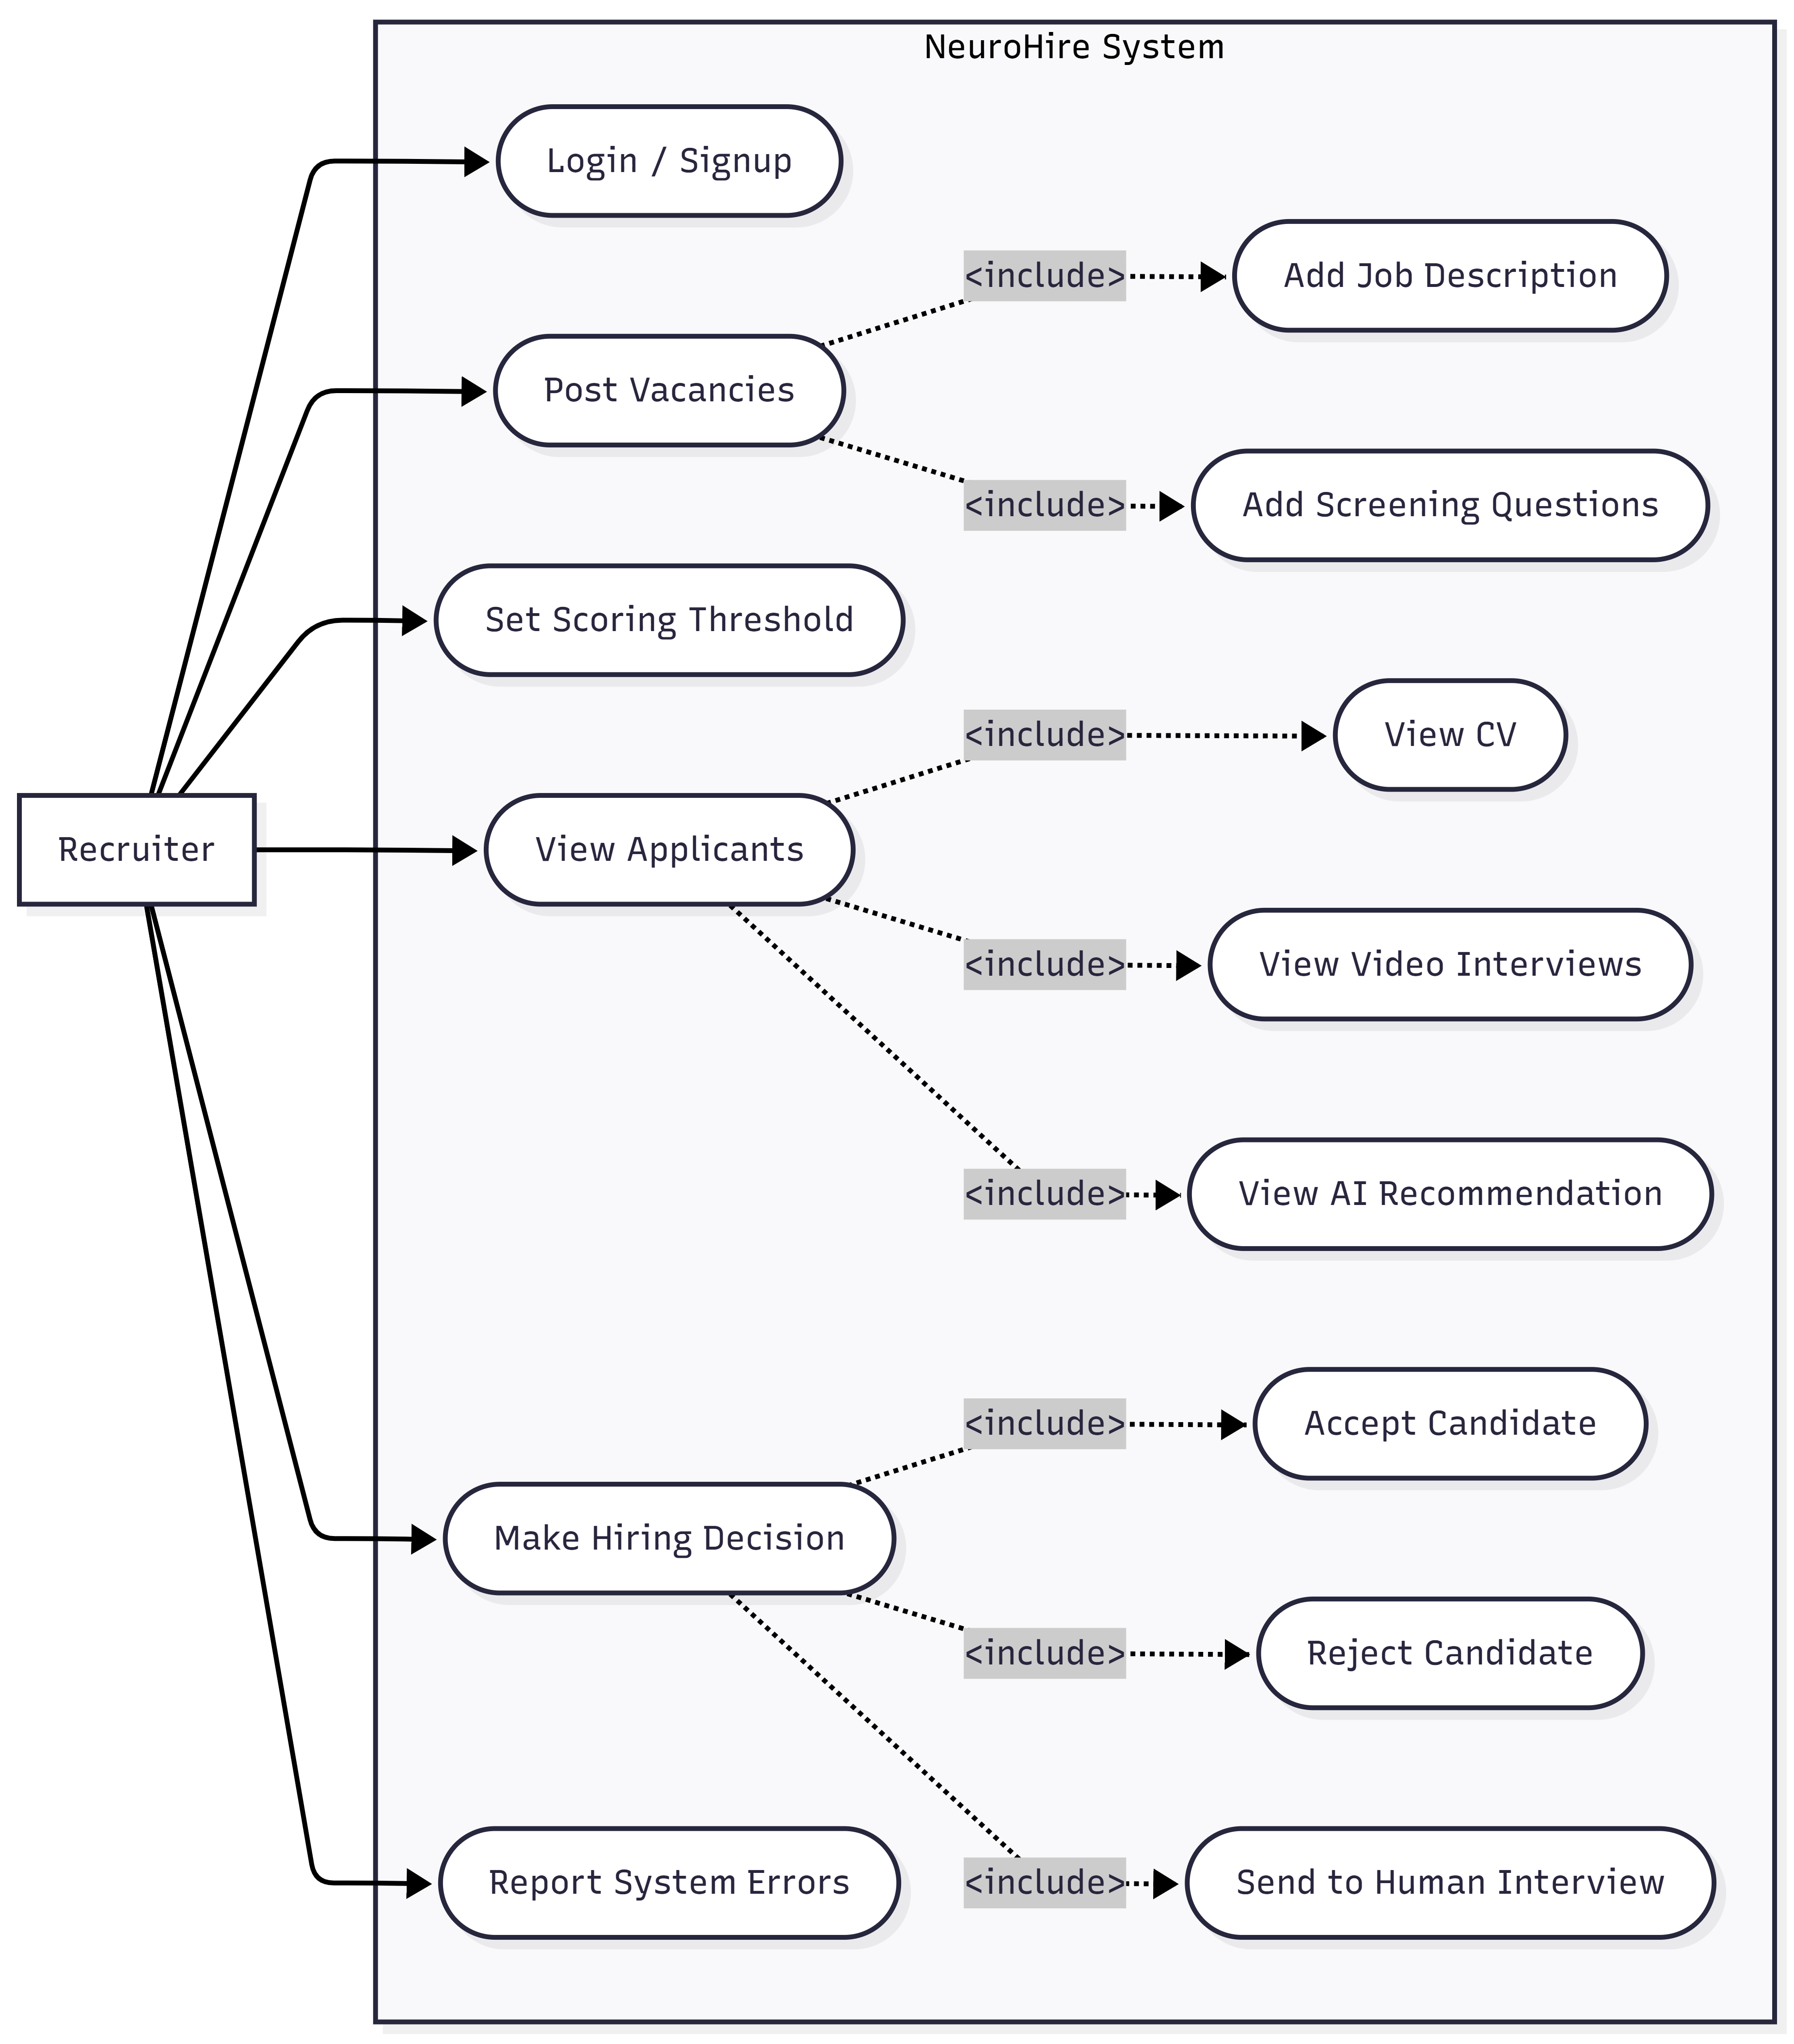
\includegraphics[width=\textwidth]{NeuroHire System Candidate-2026-04-11-141002.png}
    \caption{Recruiter Use Case Diagram}
    \label{fig:neurohire-recruiter-usecase}
\end{figure}

The use case diagram illustrates how a recruiter interacts with the NeuroHire AI Recruitment System to create job postings, evaluate applicants, and make recruitment decisions. The system supports recruiters by integrating application data, recorded interviews, and AI-generated recommendations. The process begins with \textbf{Login / Signup}, ensuring that only authorized users can access the platform. The recruiter can then \textbf{post vacancies}, which includes essential tasks such as \textbf{adding job descriptions} (defining roles, responsibilities, and requirements) and \textbf{adding screening questions} for candidate interviews; these steps are modeled using \texttt{<<include>>} relationships as they are mandatory components of job posting. 
\\
\\
The recruiter can also \textbf{set a scoring threshold}, which determines how candidates are evaluated and filtered using AI-based scoring. To assess candidates, the recruiter can \textbf{view applicants}, which includes \textbf{viewing CVs}, \textbf{viewing video interviews}, and \textbf{viewing AI recommendations}, all of which are core evaluation steps modeled as included use cases. After evaluation, the recruiter proceeds to \textbf{make hiring decisions}, which may involve \textbf{accepting candidates}, \textbf{rejecting candidates}, or \textbf{sending candidates to a human interview}, depending on the assessment results. Additionally, the recruiter can \textbf{report system errors} encountered during usage, enabling issues to be documented and resolved, thereby improving overall system reliability and performance.

\subsection*{Interaction with Company}

\begin{figure}[H]
    \centering
    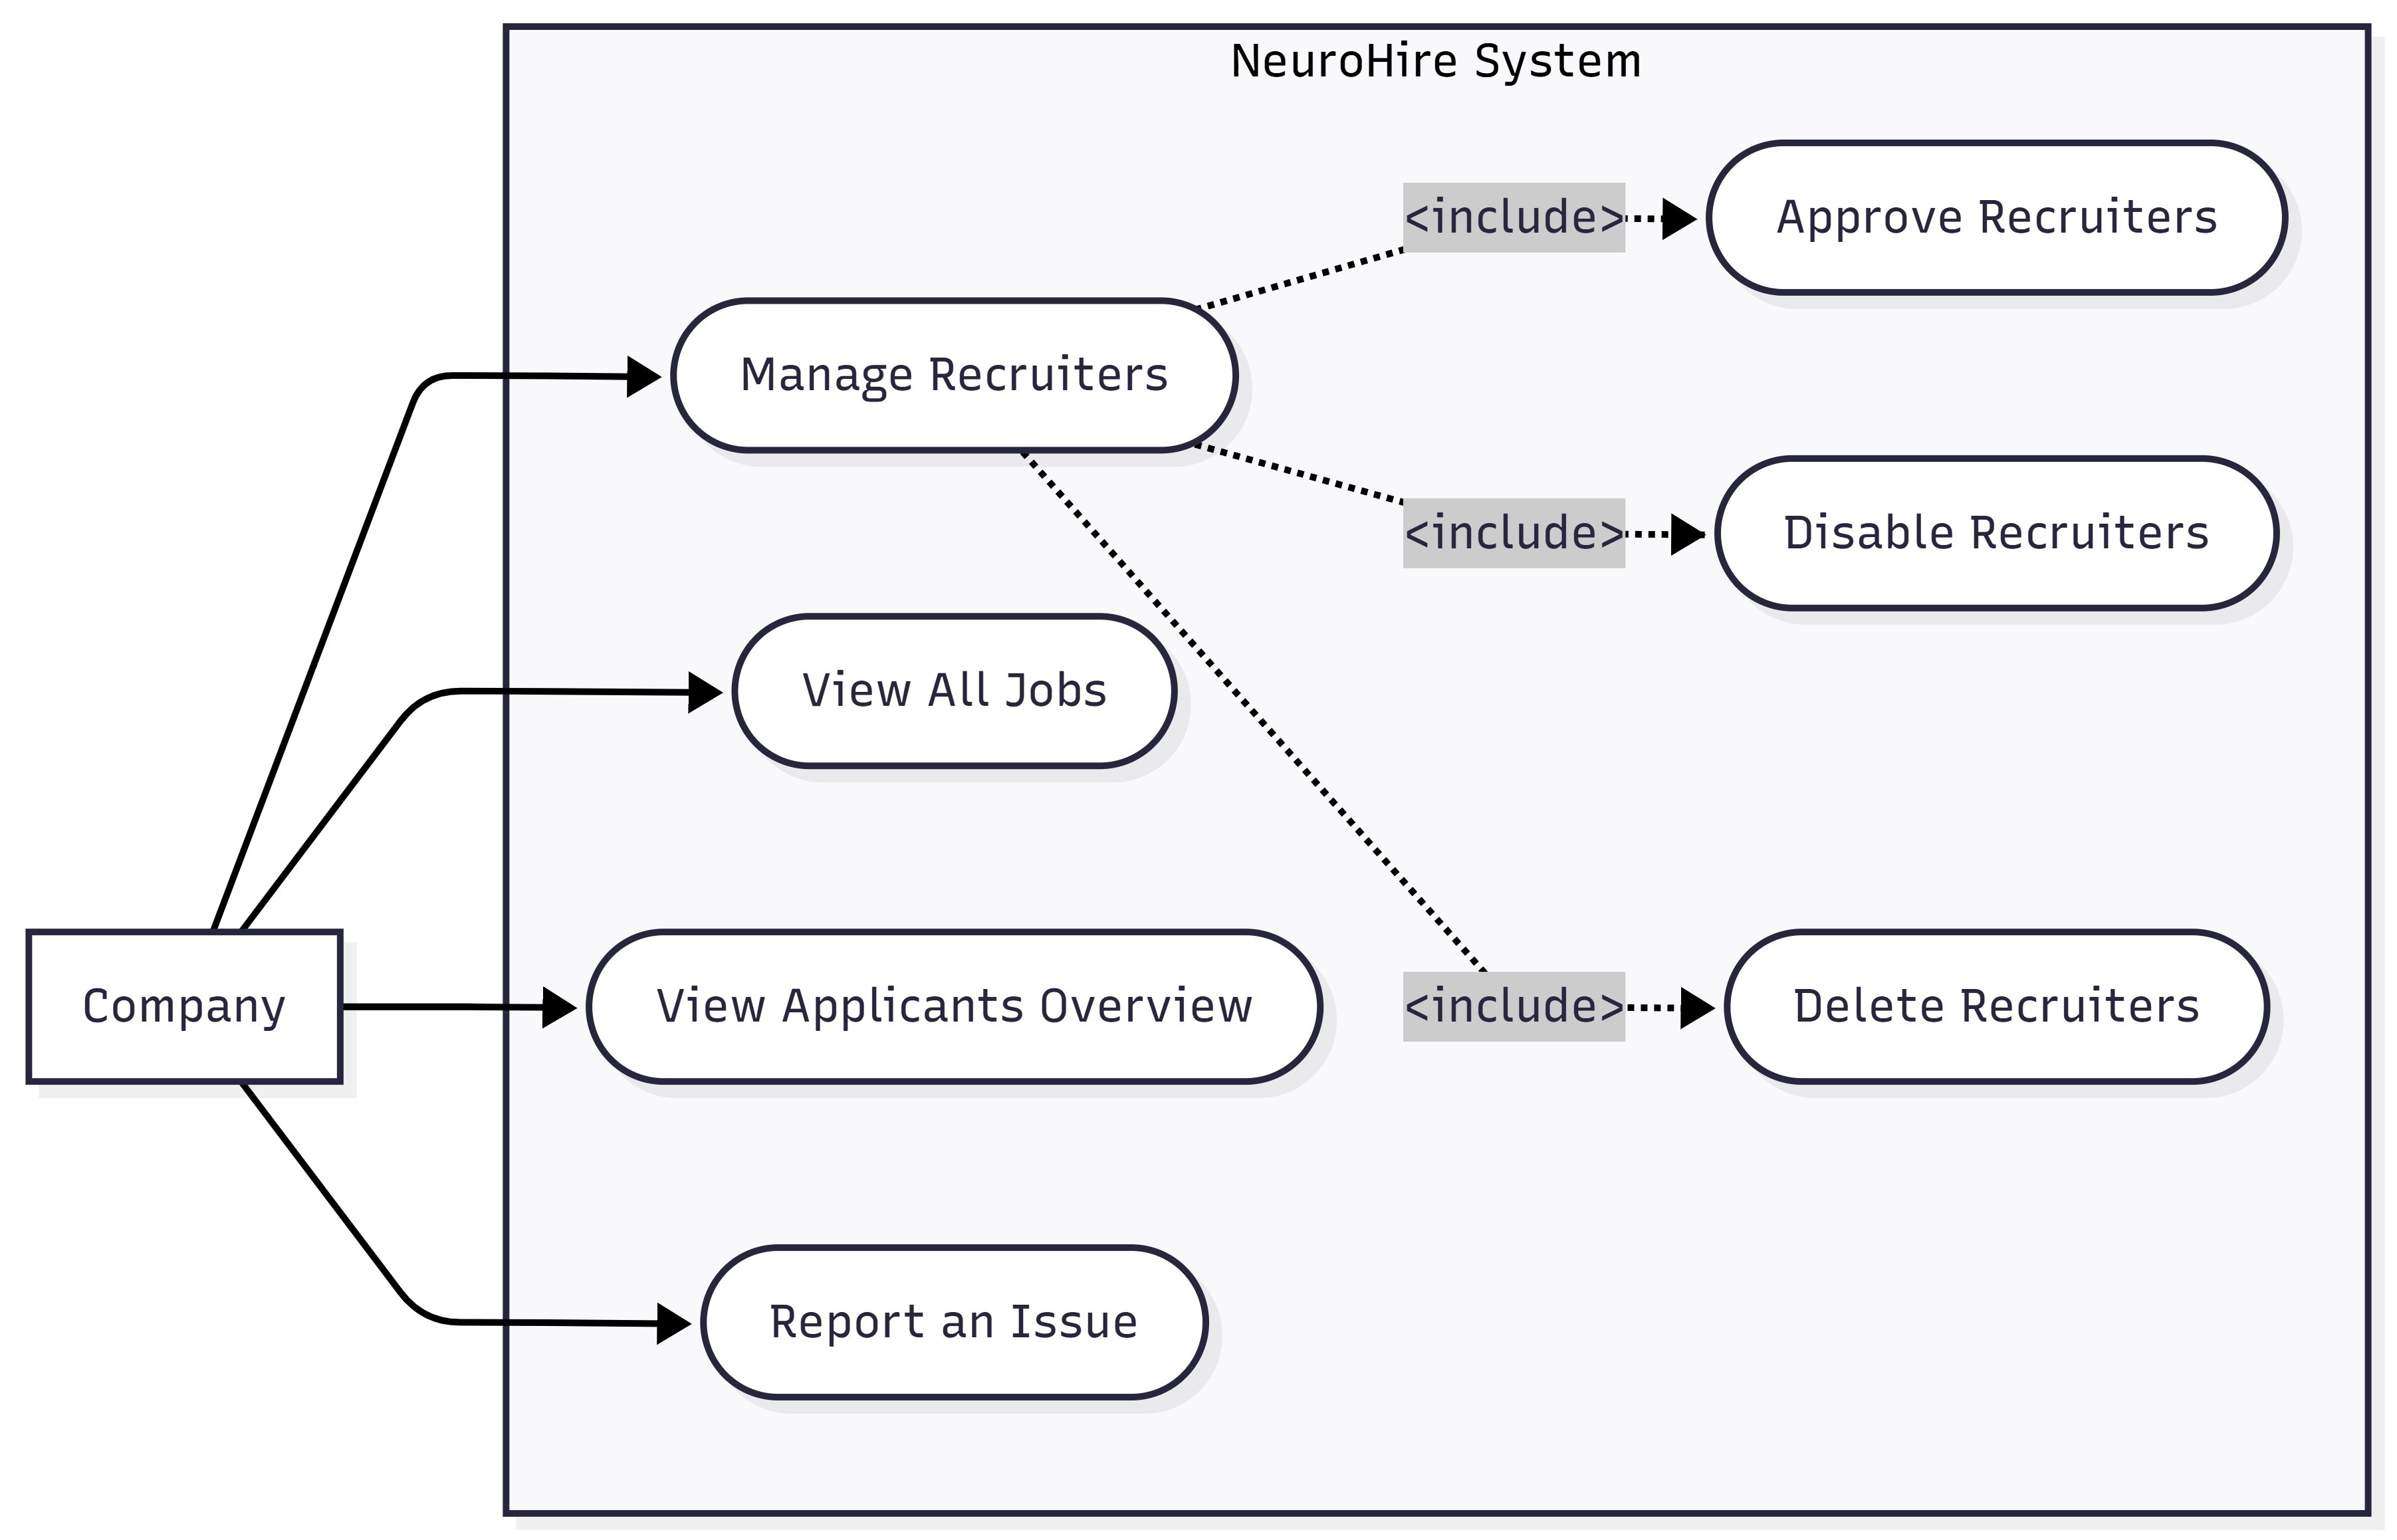
\includegraphics[width=\textwidth]{NeuroHire System Candidate-2026-04-11-143101.png}
    \caption{Company Use Case Diagram}
    \label{fig:neurohire-company-usecase}
\end{figure}

The use case diagram illustrates how a company interacts with the NeuroHire AI Recruitment System to manage recruiters, monitor job activity, and oversee the recruitment process. The system provides administrative control to ensure efficient and reliable hiring operations. A key functionality is \textbf{Manage Recruiters}, which includes actions such as \textbf{approving recruiters} to grant system access, \textbf{disabling recruiters} temporarily while preserving their data, and \textbf{deleting recruiters} permanently along with their associated information. These operations are modeled using \texttt{<<include>>} relationships, as they represent essential components of recruiter management within the system.
\\
\\
In addition to recruiter management, the company can \textbf{view all jobs} posted by its recruiters, providing complete visibility into recruitment activities. The system also offers a \textbf{view applicants overview} feature, which presents summarized data of applicants across different job postings, enabling effective monitoring of hiring progress. Furthermore, the company can \textbf{report an issue} whenever a problem is encountered, allowing system errors to be documented and resolved efficiently, thereby improving overall system reliability and user experience.



\subsection*{Interaction with Super Admin}

\begin{figure}[H]
    \centering
    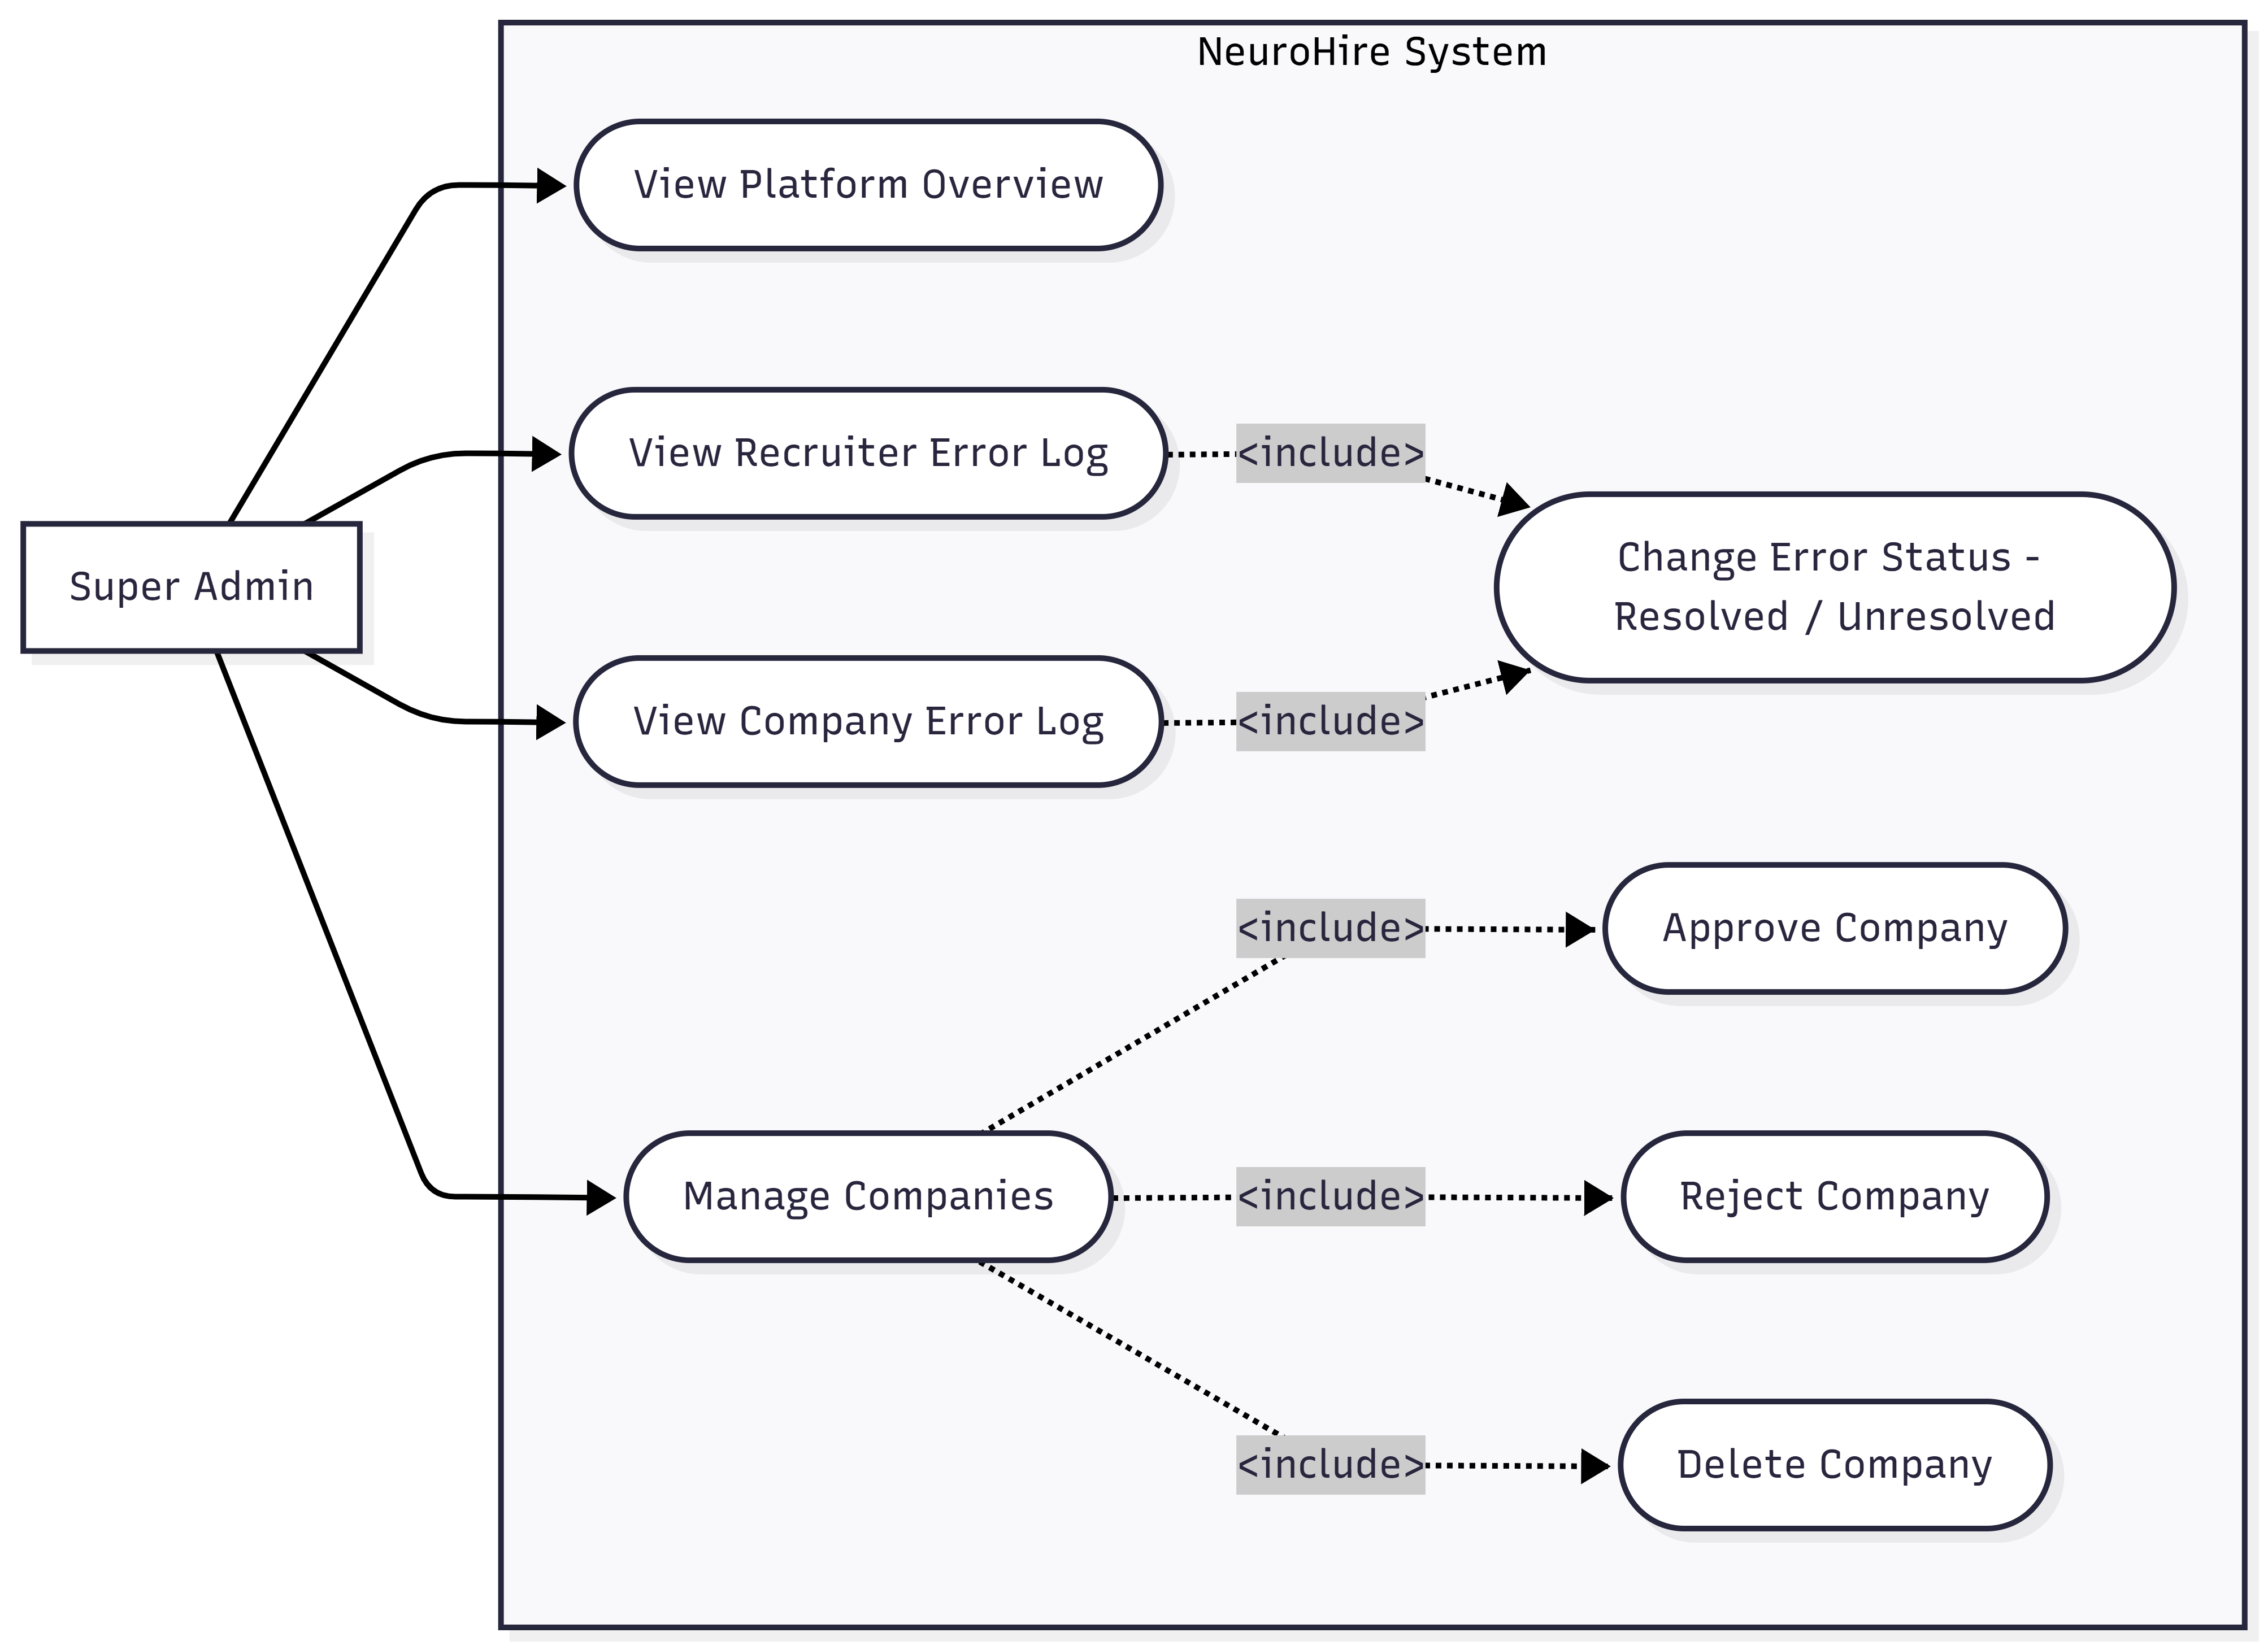
\includegraphics[width=\textwidth]{NeuroHire System Candidate-2026-04-11-143912.png}
    \caption{Super Admin Use Case Diagram}
    \label{fig:neurohire-superadmin-usecase}
\end{figure}

The use case diagram illustrates how the Super Admin interacts with the NeuroHire AI Recruitment System to monitor platform activity, manage companies, and handle system-level issues. The Super Admin acts as the highest authority, ensuring smooth system operation and administrative control. A key functionality is the ability to \textbf{view platform overview}, which provides a summary of important system metrics such as total companies, recruiters, processed candidates, and reported errors, enabling efficient monitoring of overall platform performance. Additionally, the Super Admin can \textbf{view recruiter error logs} and \textbf{view company error logs}, and perform \textbf{change error status (resolved / unresolved)} to track and manage reported issues effectively. These actions are modeled using \texttt{<<include>>} relationships, as updating error status is an essential part of error log management.
\\
\\
Another important responsibility of the Super Admin is \textbf{manage companies}, which includes operations such as \textbf{approving companies} to grant access to the platform, \textbf{rejecting companies} that do not meet requirements, and \textbf{deleting companies} permanently along with their associated data. These operations are also represented using \texttt{<<include>>} relationships, as they are core administrative functions required to maintain system integrity and control.

\section{Datasets}
This section describes the specific dataset(s) used to build our system. An appropriate snapshot of the dataset(s) is also included. Futher details, when needed, are presented in the appendix.

\section{System Diagram}
This diagram gives a high-level view of the different components of our system and the interactions between them.

\begin{figure}[h]
    \centering
    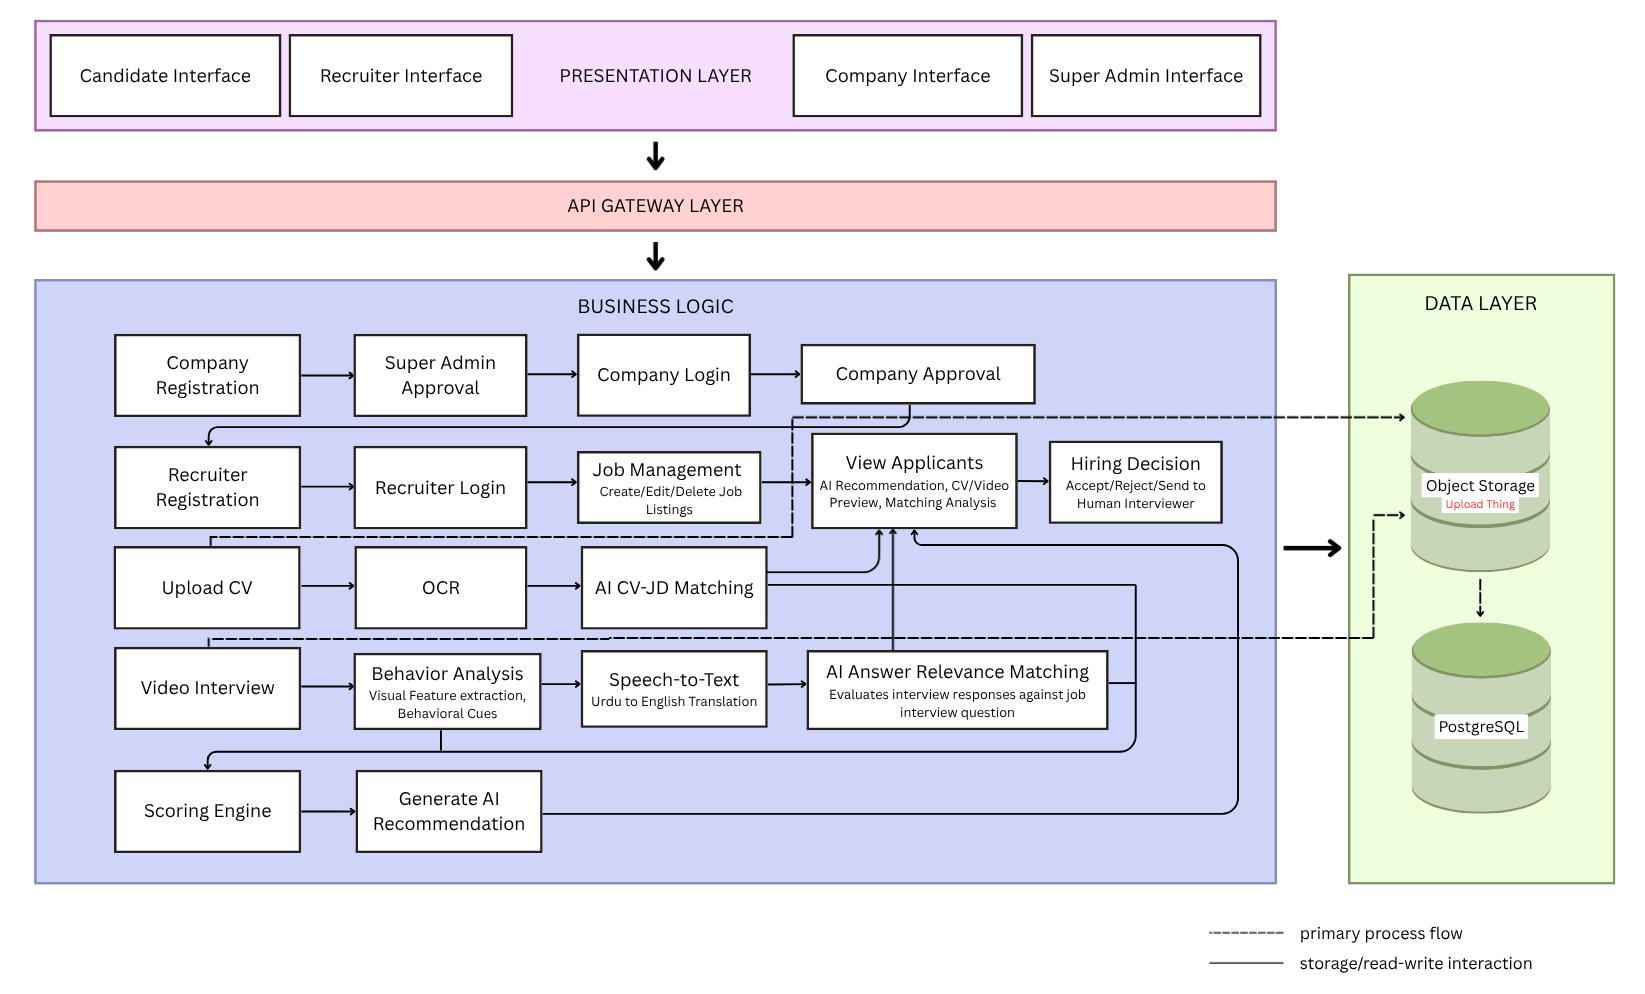
\includegraphics[width=1.05\textwidth]{system diagram.png}
    \caption{High-level system architecture of NeuroHire}
    \label{fig:system_diagram}
\end{figure}

\newpage
Each component and the particular tools, technologies, or libraries used to build it are described below:
\begin{outline}
    \1 \textbf{OCR Module:} This component is responsible for extracting textual content from uploaded CVs and resume documents. It is implemented using \textbf{OCRmyPDF} and \textbf{PaddleOCR} for optical character recognition, while \textbf{PyMuPDF} is used for PDF text extraction and document preprocessing.

    \1 \textbf{CV--JD Matching Module:} This component compares the candidate's CV with the job description to evaluate relevance and suitability. It is implemented using an \textbf{LLM-Based CV--JD Matching} approach built on \textbf{Fine-tuned LLaMA 3.2 -- 7B}.

    \1 \textbf{Speech-to-Text Module:} This component converts spoken interview responses into text for further analysis. It is implemented using \textbf{OpenAI Whisper Large v3}, which supports multilingual transcription.
    
    \1 \textbf{Answer Relevance Matching Module:} This component evaluates transcribed interview responses against job interview questions to assess answer relevance and response quality. It is implemented using \textbf{Phi-3.5 Mini Instruct (Q4\_K\_M GGUF)}.

    \1 \textbf{Behavior Analysis Module:} This component extracts visual and behavioral cues from interview videos, such as gaze direction, head movement, and facial stability. It is implemented using \textbf{OpenCV} and \textbf{MediaPipe}.

    \1 \textbf{Database Layer:} This component stores structured system data such as user accounts, job listings, applicant records, scores, and hiring decisions. It is implemented using \textbf{PostgreSQL}.

    \1 \textbf{Object Storage Layer:} This component stores unstructured files such as uploaded CVs and recorded interview videos. It is implemented using \textbf{UploadThing}.
\end{outline}

\chapter{Software Design Specification (SDS)}
\label{chap:sds}
\input{chapters/sds}

\chapter{Methodology, Experiments and Results OR Testing and Analysis}
\label{chap:results}
\input{chapters/results}

\chapter{Conclusion and Future Work}
\label{chap:outro}
\input{chapters/conclusion}

\chapter{Reflection}
\label{chap:Reflection}
\input{chapters/reflection}

\begin{appendices}

\titleformat{\chapter}[hang]{\bf\huge}{Appendix \thechapter.}{2pc}{}
  
% This appendix is optional.
\chapter{More Math}
\input{chapters/appendix-math}

% This appendix is required if the data set is not fully described in the main text.
\chapter{Data}
\input{chapters/appendix-data}

% This appendix is required if the code is not fully described in the main text.
\chapter{Code}
\input{chapters/appendix-code}
\end{appendices}

% Print the bibliography with a ToC entry and titled, "References".
\printbibliography[heading=bibintoc,title={References}]

\end{document}

%%% Local Variables:
%%% mode: latex
%%% TeX-master: t
%%% End:
